\documentclass[a4paper, 12pt, %
%draft,%
pdftex]{report} % make report->book for two sided final publishing.
%\fussy
\sloppy

\usepackage{updiss}
% Cause floats to always be below  where they are inserted as per
% Prof. de Vaal.
% \usepackage{flafter}
\usepackage{fancybox}
%%%%%%%%%

%\newcommand{\SOtwo}{\ensuremath{\mathrm{SO}_2}}
%\newcommand{\sappisaiccor}{Sappi~Saiccor}
%\newcommand{\num}[1]{\ensuremath{\fnum{#1}}}
\newcommand{\units}[1]{\ensuremath{\mathrm{#1}}}

% Title and author definitions
\title{A simplicial homology algorithm for Lipschitz optimisation}
\author{Stefan Endres} 
\degree{Master of Engineering (Chemical Engineering)} 
\department{Department of Chemical Engineering} 
\date{October 2017}

% Include directives
%\includeonly{
%front,
%progress,
% -- Text Starts --
%introduction,
%literature,
%background,
%controlanalysis, 
%current,
%controllerdesign,
%montecarlo,
%program,
%results, 
%conclusion,
% -- Appendix Entries --
% programlistings,
%parametervalues,
%testresults,
%programmingdetails,
%back
%}

\begin{document}
\maketitle
\makecoverpage

\pagestyle{plain}
\thispagestyle{plain}
\pagenumbering{roman}

\chapter*{Synopsis}\addcontentsline{toc}{section}{Synopsis}
The simplicial homology global optimisation (SHGO) algorithm is a general purpose global optimisation algorithm based on applications of simplicial integral homology and combinatorial topology. SHGO approximates the homology groups of a complex built on a hypersurface homeomorphic to a complex on the objective function. This provides both approximations of locally convex subdomains in the search space through Sperner's lemma (\citeauthor{Sperner1928}, \citeyear{Sperner1928}) and a useful visual tool for characterising and efficiently solving higher dimensional black and grey box optimisation problems. This complex is built up using sampling points within the feasible search space as vertices. The algorithm is specialised in finding all the local minima of an objective function with expensive function evaluations efficiently which is especially suitable to applications such as energy landscape exploration. SHGO was initially developed as an improvement on the topographical global optimisation (TGO) method first proposed by \citeauthor{Torn1986} (\citeyear{Torn1986, Torn1990, Torn1992}). It is proven that the SHGO algorithm will always outperform TGO on function evaluations if the objective function is Lipschitz smooth. In this paper SHGO is applied to non-convex problems with linear and box constraints with bounds placed on the variables. Numerical experiments on linearly constrained test problems show that SHGO gives competitive results compared to TGO and the recently developed Lc-DISIMPL algorithm (\citeauthor{Paul2016}, \citeyear{Paul2016}) as well as the PSwarm and DIRECT-L1 algorithms. Furthermore SHGO is compared with the TGO, basinhopping (BH) and differential evolution (DE) global optimisation algorithms over a large selection of black-box problems with bounds placed on the variables from the SciPy (\citeauthor*{scipy}, \citeyear{scipy}) benchmarking test suite. A Python implementation of the SHGO and TGO algorithms published under a MIT license can be found from \url{https://bitbucket.org/upiamcompthermo/shgo/}.
\bigskip

\noindent \textbf{SLEUTELWOORDE:} Global optimisation, SHGO, Computational homology
\begin{flushleft}\bf{Mathematics Subject Classification (2010)} \normalfont 90C26 Nonconvex programming, global optimisation
\end{flushleft}

% Local Variables: 
% TeX-master: "thesis" 
% End:



%\input{acknowledgements.tex}

\tableofcontents
\newpage
\listoffigures
\newpage
\listoftables
\newpage
%\chapter*{Nomenclature}
%\printglossary
\newpage

% Local Variables:
% TeX-master: "thesis"
% End:


% Page numbering: Start at 1

\pagestyle{headings}
\setcounter{page}{1}
\pagenumbering{arabic}

%\section{Introduction}
\chapter{Introduction}
\section{Objective function statement and nomenclature}
Consider a general optimisation problem of the form
\begin{align} \nonumber
\underset{\mathbf{x}}{\textrm{min}} ~&f (\mathbf{x}) \\ \label{eq:gen_op}
\textrm{s.t.}~ &\mathbf{g} (\mathbf{x}) \geq 0
\end{align}
The continuous real objective function $f(\mathbf{x})$ maps a vector of dimension $n$ to a scalar value. It can be either smooth or non-smooth depending on the local minimisation method used. The variables $\mathbf{x}$ are assumed to be bounded. In this dissertation we mainly consider real, smooth, but not necessarily convex functions with linear constraint functions. In addition it is assumed that the objective function has a finite number of local minima
\begin{equation} \label{eq:objfun}
f : \mathbb{R}^n \rightarrow \mathbb{R}
\end{equation}
$\mathbf{g}$ maps the set of linear constraints
\begin{equation} \label{eq:gcons}
\mathbf{g} :  [\mathbf{l}, \mathbf{u}]^n  \rightarrow \mathbb{R}^m
\end{equation}
for example if lower and upper bounds $l_i$ and $u_i$ are implemented for each variable then we have an initially defined hyperrectangle 
\begin{equation}
\mathbf{x} \in \Omega \subseteq  [\mathbf{l}, \mathbf{u}]^n~=~[l_1,~u_1]~\times~[l_2,~u_2] ~\times~\dots~\times~[l_n,~u_n] \subseteq  \mathbb{R}^n
\end{equation}
 where $\Omega$ is the limited feasible subset excluding points outside the bounds and constraints. 
\begin{equation} \label{eq:omega}
\Omega = \{ \mathbf{x} \in   [\mathbf{l}, \mathbf{u}]^n ~|~ \mathbf{g}_i (\mathbf{x} ) \geq 0, \forall i =1, \dots, m\}
\end{equation}
Since the constraints in $\mathbf{g}$ are linear the set $\Omega$ is always a compact space.

In the development of SHGO several concepts from algebraic and combinatorial topology \citep{Henle1979} are required. The following definition was adapted from \citet[p. 9]{Hatcher2011} 

\begin{definition}
A \textbf{$\mathbf{k}$-simplex} is a set of $n+1$ vertices in a convex polyhedron of dimension $n$. Formally if the $n+1$ points are the $n+1$ standard $n+1$ basis vectors for  $\mathbb{R}^{(n+1)}$. Then the $n$-dimensional $k$-simplex is the set
 $$ 
S^{n}=  \left\{ (t_1 ,\dots , t_{n +1})  \in\mathbb{R}^{n+1} ~|~ \sum^{n +1}_1 t_{n +1}  = 1,  t_i \geq  0  \right\}
$$

%Concretely, if the n points are the n standard
%nbasis vectors for R , then their join is the (n − 1) dimensional simplex
 %∆n−1 =  \{ (t_1 , ···  , t_n)  \in R  n || t1  + ···  +  tn  = 1 and ti ≥  0  }
\end{definition}
For example, a 2-simplex is a triangle and a 3-simplex is a tetrahedron. We will use the following combinatorial definition of a simplicial complex \citep[p. 107]{Hatcher2011}
\begin{definition}
A \textbf{simplicial complex}  $\mathcal{H}$  is a set $\mathcal{H}^0$  of vertices together with sets $\mathcal{H}^n$  of $n$-simplices, which are ($n + 1$)-element subsets of $\mathcal{H}^0$. The only requirement is that each ($k + 1$)-elements subset of the vertices of an $n$-simplex in $\mathcal{H}^n$ is a $k$-simplex, in $\mathcal{H}^k$ .
\end{definition}
Thus each  $n$-simplex  has $n + 1$ distinct vertices, and no other $n$-simplex has this same set of vertices.

In this publication the $\mathcal{H}$ symbol will be used to represent a (finite) simplicial complex rather than the more standard $\Delta $ to avoid confusion with the difference and Laplacian operators common in optimisation. The superscript $\mathcal{H}^k$ represents the subset of $k-$dimensional simplices where for an $n$ dimensional problem the highest dimensional $k-$simplex contains $n + 1$ vertices. Finally we define a $k$-chain \citep{Henle1979}

\begin{definition}
A $\mathbf{k}$-\textbf{chain} is a union of simplices.
\end{definition}
For example a 0-chain is a set of vertices, a 1-chain is a set of edges and a 2-chain is a set of triangles. $C(\mathcal{H}^k)$ denotes a $k-$chain of $k-$simplices. A vertex in $\mathcal{H}^0$ is denoted by $v_i$. If $v_i$ and $v_j$ are two endpoints of a directed edge in $\mathcal{H}^1$ from $v_i$ to $v_j$ then the symbol $\overline{v_i v_j}$ represents the edge so that it is bounded by the $0-$chain $\partial \left( \overline{v_i v_j} \right) = v_j - v_i$ and similarly for an edge directed from $v_j$ to $v_i$, we have, $\partial \left( \overline{v_j v_i} \right) = \partial \left( - \overline{v_i v_j} \right) = v_i - v_j$. Higher dimensional simplices can be represented and directed in a similar manner, for example a triangle consisting of three vertices $v_i, v_j$ and $v_k$ directed as $\overline{v_i v_j v_k}$  has the boundary of directed edges $\partial \left( \overline{v_i v_j v_j} \right)  = \overline{v_i v_j} + \overline{v_j v_k} + \overline{v_j v_i}$.

\section{Multimodal objective functions and local minima mapping}
Non-convex problems are commonly solved using global optimisation methods. One such example is the topographical global optimisation (TGO) method \citep{Henderson2015, Torn1986, Torn1990, Torn1992} which is a clustering algorithm that finds several local minima from which the (probable) global minimum is found. It is often desirable to find all the local minima of the objective function for example in applications such as energy landscape exploration of potential models wherein mapping the local minima of the potential functions can provide valuable insights into the system. Algorithms such as the basin-hopping global optimisation algorithm are typically used to find these points \citep{Wales2015}.




% for example in phase equilibria problems where it is required to map the local minima of the Gibbs energy surface to find all the phases in equilibrium using methods described in \citet{Zhang2011} \citep{Michelsen1982, Michelsen1982a, Mitsos2007, Mitsos, Bollas2009, Bollas2009b}.

The graph extracted from the topographical global optimisation (TGO) \citep{Henderson2015, Torn1986, Torn1990, Torn1992} topograph (as described in \Cref{sec:TGO}) is unsatisfactory in some ways. Primarily because several starting points in the same locally convex domain can be generated even when enough information from the objective function sampling is known to prevent this from occurring. This leads to superfluous function evaluations in the local minimisation step of the algorithm. Contrary to intuition, this problem is exacerbated by increasing the number of initial sampling points used in the algorithm as demonstrated in \Cref{sec:TGO}. This can lead to a very large number of function evaluations required to solve the problem. In particular in multimodal energy surfaces where the local minima can often be located in short distances relative to the search space \citep{Zhang2011} and thus requires a large number of initial sampling to locate all these domains. Some shortcomings in using the TGO method to map local minima are:
\begin{itemize}
\item Geometric information available from the sampling points is being disregarded by the graphs built up using only the Euclidean distance metric.
\item Knowledge of the number and location of local minimisers in a given sampling set is not being used to the full extent.
\item More than one minimiser might be produced in the same locally convex domain and there is no guarantee that a minimiser set produced by TGO will be in the locally convex domains of all local minima even if the number of local minima is known and a minimiser set of this cardinality is produced.
\end{itemize}

By constructing a directed simplicial complex it will be shown that the simplicial homology global optimisation (SHGO) algorithm does not produce superfluous starting points for the class of all Lipschitz smooth functions resulting in more efficient performance for these problems compared to TGO. The directed complex is also used to approximate the homology group of the objective function hypersurface which, using integral homology version of the Invariance Theorem \citep{Henle1979}, allows for efficient mapping of optimisation problems where the number of local minima is known \it{a-priori}\normalfont. %For example in phase equilibria problems where the maximum number of minima is known through the Gibbs phase rule and in certain problems the exact number of phases is known \it{a-priori} \normalfont \citep{Zhang2011}.

\section{Derivative-free methods for Lipschitz optimsation problems}
Both the SHGO and TGO algorithms only make use of function evaluations without requiring the derivatives of objective functions. This makes them applicable to black-box global optimisation problems. A recent review and experimental comparison of 22 derivative-free optimisation algorithms by \citet{Rios2013} concluded that global optimisation solvers solvers such as TOMLAB/MULTI-MIN, TOMLAB/GLCCLUSTER, MCS and TOMLAB/LGO perform better, on average, than other derivative-free solvers in terms of solution quality within 2500 function evaluations. Both the TOMLAB/GLCCLUSTER and MCS \citep{Huyer1999} implementations are based on the well-known DIRECT (DIviding RECTangle) algorithm \citep{Jones1993}.
 
The DISIMPL (DIviding SIMPLices) algorithm was recently proposed by \citet{Paul2014b}. The experimental investigation in \citet{Paul2014b} shows that the proposed simplicial algorithm gives very competitive results compared to the DIRECT algorithm. DISIMPL has been extended in \citet{paulavivcius2014simplicial, Paul2014a}. The Gb-DISIMPL (Globally-biased DISIMPL) was compared in \citet{Paul2014a} to the DIRECT and DIRECTl methods in extensive numerical experiments on 800 multidimensional multiextremal test functions.

In a recent adaption of DISIMPL for linearly constrained optimisation problems, Lc-DISIMPL \citep{Paul2016} showed extremely competitive results compared to the PSwarm \citep{Vaz2008} and DIRECT-L1 algorithms \citep{finkel2003direct}. In particular the Lc-DISIMPL-v algorithm was shown to solve the problems in a fewer number of function evaluations on average and was the only algorithm to converge on all of the test problems. In this dissertation both the SHGO and TGO algorithms were tested on the same problem set and the results are compared to the data from \citet{Paul2016} which also contains results on the PSwarm \citep{Vaz2008} and DIRECT-L1 algorithms \citep{finkel2003direct}.

The DISIMPL algorithm is the most similar to SHGO in the sense that both make use of a simplicial complex. DISIMPL uses a simplicial complex in a  spatial partitioning of the initial search space. Since the geometric structure of the two algorithms are related, it is reasonable to expect some theoretical relation of its properties. In particular the graph structure in the DISIMPL-v algorithm \citep{Paul2016} can be used to build the directed simplicial complex used by SHGO. In \Cref{sec:shgo} we also show how some of the same principles developed for SHGO can also be applied in the DISIMPL-v algorithm since the same information is readily available to the algorithm.
 
\section{Structure}
The TGO method is briefly reviewed in \Cref{sec:TGO} closely following the formalism developed by \citet{Henderson2015}. In \Cref{sec:motivation} we provide numerical examples of TGO which is then used as an informal experimental motivation for extending the algorithm. These two chapters are important for continuity and understanding of the improved features of SHGO, in particular \Cref{def:optpool} which will be used as a performance criterion. In \Cref{sec:atgo} we present the most immediately apparent extension of TGO and illustrate the shortcomings of that approach. The new SHGO method is then formally presented in \Cref{sec:shgo}. In \Cref{sec:results} we provide experimental results of linearly constrained problems comparing the SHGO, TGO, Lc-DISIMPL \citep{Paul2016}, PSwarm \citep{Vaz2008} and DIRECT-L1 \citep{finkel2003direct} algorithms. Furthermore SHGO is compared with the TGO, basinhopping (BH) and differential evolution (DE) global optimisation algorithms over a large selection of black-box problems from the SciPy (\citeauthor*{scipy}, \citeyear{scipy}) global optimisation benchmarking test suite. We conclude with various recommendations for possible further improvements of SHGO.

A very quick introduction to SHGO, along with installation and usage instructions can be found on the public website for the project: \href{https://stefan-endres.github.io/shgo/}{https://stefan-endres.github.io/shgo/}

%\section{TGO}
\chapter{Topographical Global Optimisation (TGO)}  \label{sec:TGO}
The Topographical Global Optimisation (TGO) was originally conceived by \citet{Torn1990} and Henderson et al. \citep{Henderson2015, Henderson2016} introduced new formalisms and empirical methods to determine hyperparameters described in this section. \citet{Henderson2015} also presents the algorithm in an introductory fashion. It is in essence an iterative clustering algorithm that maps the hypersurface of the objective function into a topography matrix (called a $t$-matrix) and then finds a certain number of starting points referred to as local minimisers. A local search using the local minimisers as starting points is then used to find each minimum from which the global minimum is finally calculated. \citet{Henderson2015} used the feasible direction interior-point method proposed by \citet{Herskovits1998} in this step. The feasible direction interior-point method allows for minimisation of problems with linear and/or nonlinear equality constraints; an extension by \citet{Henderson2015} of the original applications of \citet{Torn1990}. The TGO method consists of three steps:
\begin{enumerate}
\item Uniform random sampling generation of $N$ points in the search space.
\item Construction of the topograph, which is a directed graph with the sampled points as vertices on a $k$-nearest neighbours basis with the direction of the arc directed towards a point with a larger function value.
\item Local minimisation of topograph minimisers. 
\end{enumerate}

\section{Step 1: Random Sampling Point generation} \label{sec:tgo1}
In order to generate the uniform sampling points within $\Omega$ the deterministic Sobol sequence is used in this dissertation \citep{Henderson2015, Sobol1967}. Other possible low discrepancy sequences such as the Halton and Van der Corput sequences \citep{zbMATH03440485} can also be used in this step. An efficient Gray code implementation was proposed by \citet{Antonov1979} wherein a single XOR operation for each dimension can be used to find the next sampling point in the sequence $x_{n,i}=x_{n-1,i} \oplus v_{k,i}. \,$ An adaptation of this method is available in the open source Python library UQToolbox\citep{Bigoni2016}. The Sobol sequenced points are generated within the $n$ dimensional hypercube $ [0, 1]^n~\in ~\mathbb{R}^n $, providing a uniform distribution on the hypersurface within this space. In the current implementation this set of points is stretched across the lower and upper bounds to form the hyperrectangle $[\mathbf{l}, \mathbf{u}]^n = [l_1,~u_1] \times~[l_2,~u_2]  \times \dots \times [l_n,~u_n] \subseteq  \mathbb{R}^n$. The subset of feasible points contained in $\Omega$ is found by discarding any points lying outside the constraints $ \mathbf{g}(\mathbf{x}) > 0$.

\section{Step 2:  Construction of the topograph} \label{sec:tgo2}
The topograph is constructed from the generated sampling points within $\Omega$. From the topograph several global minimisers in $f$ are found using the definitions developed in this chapter which are then used as starting points for local minimisation routines. First $N$ points are selected from the uniformly generated sequence of points within the feasible domain of $\Omega \subset \mathbb{R}^n$. Points generated by the sequence that lie outside the constraints are excluded. The points are denoted by $\bold{p}_i, i = 1, 2, 3 \dots N$. Next for each point $\bold{p}_i $ a reference list is constructed by ordering the other $N -1$ points from their nearest to farthest Euclidean distances. These ordered lists make up the rows of the topography matrix (or topograph). Furthermore, for some point $\bold{p}_j \in \left\{1, 2, 3 \dots (N - 1)\right\}$ in the row with the first entry $\bold{p}_i $, a sign is assigned as follows:
\[ \textrm{sign} (\bold{p}_j) = \begin{cases} 
       f(\bold{p}_j)  \geq f(\bold{p}_i) & \rightarrow +\\
       f(\bold{p}_j) <  f(\bold{p}_i)  & \rightarrow  -
   \end{cases}
\]
In order to demonstrate this construction we will define this ordered list in such a way that the increasing indices represent an ordered list of the nearest points to $\bold{p}_1$, that is $\left\| \mathbf{\bold{p}_{i }} - \mathbf{\bold{p}_{i + 1}} \right\|  \leq \left\| \mathbf{\bold{p}_{i+1 }} - \mathbf{\bold{p}_{i + 2}} \right\|   \forall i$ .  Suppose for example that $f(\bold{p}_2)  \geq f(\bold{p}_1) $,  $f(\bold{p}_3 )< f(\bold{p}_1)$ and $f(\bold{p}_N ) \geq f(\bold{p}_1)$, the resulting topograph with the first row known is:

\begin{equation} \label{eq:tmatrix}
t \textrm{-} \textrm{matrix} =
%  pmatrix bmatrix  Bmatrix  vmatrix  Vmatrix
    \begin{pmatrix}[c|cccc]
  \bold{p}_1 & +\bold{p}_2 		& -\bold{p}_3				& \dots 		&  +\bold{p}_N\\
   \vdots &    \vdots 	&     \vdots 	& \ddots 	&  \vdots\\
   \bold{p}_N & \bold{p}_j 			&  \dots			&  \bold{p}_j 		&  \bold{p}_j \\ 
    \end{pmatrix}
\end{equation}
Note that the remaining rows (represented by unknown points and signs $\bold{p}_j$) are constructed similarly to the first row for every $\bold{p}_i$ row. The topography matrix can be interpreted as a directed graph, where the signs represent the directed arcs on the graph. It should also be noted that if $\mathbf{g}$ contains non-linear constraints then the graphs produced by the topograph may be connected across disconnected and/or non-convex subspaces of $\Omega$.  Example 1 in \Cref{sec:motivation} demonstrates the construction of the topograph numerically.

Given and integer $1 \leq k \leq (N -1)$, the $N \times k$  submatrix obtained by considering only the $k$-nearest neighbours is called the $k$-$t$-matrix. For example for $k =1 $:
\begin{equation}
1 \textrm{-}t \textrm{-} \textrm{matrix} =
%  pmatrix bmatrix  Bmatrix  vmatrix  Vmatrix
    \begin{pmatrix}[c|c]
  \bold{p}_1    & +\bold{p}_2\\
   \vdots   &   \vdots 	\\
   \bold{p}_N  & \bold{p}_j 		\\ 
    \end{pmatrix}
\end{equation}
for $k =2 $:
\begin{equation}
2 \textrm{-} t \textrm{-} \textrm{matrix} =
%  pmatrix bmatrix  Bmatrix  vmatrix  Vmatrix
    \begin{pmatrix} [c|cc]
    \bold{p}_1   &  +\bold{p}_2 		& -\bold{p}_3			\\
    \vdots   &    \vdots 	&     \vdots 	\\
    \bold{p}_N  & \bold{p}_j  &  \bold{p}_j		\ \
    \end{pmatrix}
\end{equation}
and so forth. The  $k$-$t$-matrix is a representation of its $k^+$-topograph where every row forms a directed subgraph.

The following definitions adapted from \citet{Henderson2015} are used to find the global minimisers of the objective function
\begin{definition} \label{def:tgo1}
Given an integer $1 \leq k \leq (N -1)$, the $i$th row of the $k$-$t$-matrix is said to be a positive row, if all its elements have a plus sign. That is iff $ f(\bold{p}_j)  \geq f(\bold{p}_i)  ~\forall j$.
\end{definition}

\begin{definition} \label{def:tgo2}
 Given an integer $1 \leq k \leq (N -1)$,  a sampling point $\bold{p}_i$ has a positive reference in the $k$-$t$-matrix, if there exists $j \neq i$ such that (a) the $j^{th}$ row of the $k$-$t$-matrix is a positive row and (b) the number $+i$ is an element of this $j^{th}$ row. 
\end{definition}

\begin{definition} \label{def:tgo3}
Given an integer $1 \leq k \leq (N -1)$, the sample point $\bold{p}_i$ is called a local minimiser of $f$ in the $k^+$-topograph if the $i^{th}$ row of the $k$-$t$-matrix is a positive row.
\end{definition}

\begin{definition} \label{def:tgo4}
Given an integer $1 \leq k \leq (N -1)$, the sample point $\bold{p}_i$ is a global minimiser of $f$ in the $k^+$-topograph if $\bold{p}_i$ is a local minimiser of $f$ in the $k^+$-topograph and, in addition, $\bold{p}_i$ has no positive references in the $k$-$t$-matrix. 
\end{definition}

The following propositions can be readily demonstrated to show the consistency of the aforementioned definitions \citep{Henderson2015}.

\begin{proposition}  
Given an integer $1 \leq k \leq (N -1)$, the sample point $\bold{p}_i$ is a global minimiser of $f$ in the $k^+$-topograph if and only if the sample point $\bold{p}_i$ is the only minimiser of $f$ in the $k^+$-topograph which is global.
\end{proposition}

\begin{proposition} 
Given an integer $1 \leq k \leq (N -1)$, then the $i$th row of $k$-$t$-matrix is the only positive row of this matrix if and only if the sample point $\bold{p}_i$ is the only minimiser of $f$ in the $k^+$-topograph which is global.
\end{proposition}

\begin{corollary}
 Given an integer $1 \leq k \leq (N -1)$, if the sample point $\bold{p}_i$ is the only local minimiser of $f$ in the $k^+$-topograph, then $\bold{p}_i$ is a global minimiser of $f$ in this graph.
\end{corollary} 

In this publication we will use the paradigm that all local minimisers of $f$ in the $k^+$ -topograph will be used for the local search (Paradigm 2.2 in \citet{Henderson2015}). As described in \citet{Torn1992} the number of local minimisers of $f$ in the $k^+$-topograph is greater than or equal to number of global minimisers in the topograph. We will therefore employ the following definition
\begin{definition}  \label{def:tgo5}
Given an integer $1 \leq k \leq (N -1)$, the minimiser pool $\mathcal{M}^k$ is the set containing all local minimisers $\bold{p}_i$ in the in the $k^+$-topograph. The total number of starting points used in the local search step is equal to the cardinality of the minimiser pool $|\mathcal{M}^k|$. 
\end{definition}

%
The entire point of using $k$-$t$-matrices is because a $t$-matrix will always have at most one local (and thus global) minimiser. This is undesirable since this sampling point is not necessarily the starting point closest to the true global minimum of the objective function. \citet{Henderson2015} developed a semi-empirical formula producing an integer value $k_c$ which is used as an estimate for the optimal value for the integer $k$.
 
 
\section{Step 3: Local minimisation} \label{sec:tgo3}
Each of the minimisers from the  $k_c$-$t$-topograph is now used as a starting point in a local minimisation routine. The resulting minima are used to find the global minimum. Conceivably various local optimisation routines can be used to address a broad class of optimisations problems. For problems with non-linear inequality constraints \citet{Henderson2015} used the feasible direction interior-point method proposed by \citet{Herskovits1998} minimising the objective function $f$ subject to the set of inequality constraint functions $\mathbf{g}$ using the minimiser set as the initial starting points for the algorithm. An algorithm used to solve the feasible direction interior-point method using the set of starting points calculated in step 2 is presented in detail by \citet{Henderson2015}. 

In this publication we will mainly be using the sequential least squares quadratic programming optimisation algorithm (SLSQP) contained in the SciPy library originally developed by Kraft \citep{Kraft1988, Kraft1994}. The Python implementation of the TGO algorithm published under an open source licence uses this algorithm as implemented in the SciPy library \citep{TGOpy, scipy}.


%\section{Motivation}
\chapter{Motivation and a one-dimensional prelude} \label{sec:motivation}

In this section we will demonstrate how the Euclidean distance criterion in the TGO method disregards useful information about the (approximate) geometry of the objective function and we show how known information can be used effectively both in global optimisation and in mapping the local minima of objective functions as efficiently as possible. We also show how two important hyperparameters used by TGO, namely the number of sampling points $N$ and the choice of $k$ can be iteratively selected by intelligently exploiting information known from the topograph. This draws parallels to other works on iterative versions of TGO (I-TGO) \citep{Torn1996} trying to extract information from black-box objective functions. The informal, but intuitive ideas developed here will later be extended more rigorously to higher dimensional surfaces. Note that from Equation (\ref{eq:omega}) $\Omega$ is always a compact space, this fact is important in several proofs used in this Section. %, in \Cref{sec:shgo} we show that these ideas extend naturally to non-convex sets of $\Omega$ iff they contain any disconnected compact subspaces. %$ then if certain assumptions are made about the sampling sequence. 
\paragraph{Example 1}Consider the following objective function
\begin{equation} \label{eq:test1}
\underset{x}{\min} ~f(x) = \frac{\sin(x)}{x}, ~ x \in  \Omega = [1, 20]
\end{equation}
In this instance of the bounded optimisation problem there are 3 local minima which we will try to map in as few function evaluations as possible. 

Following the TGO procedure we start by generating low-discrepancy sampling points. The first $N = 10$ points in the 1-dimensional Sobol sequence is given by
$\mathcal{P} = \{
   p_{1}   =   1.0,  
   p_{2}   =   10.5,    
   p_{3}   =   15.25,   
   p_{4}   =   5.75,
   p_{5}   =   8.125,   
   p_{6}   =   17.625,    
   p_{7}   =   12.875, 
   p_{8}   =   3.375,   
   p_{9}   =   4.5625,   
   p_{10}   =   14.0625 \} \subset \Omega $.
After mapping the objective function at the set of sampling points    
\begin{equation}
f:
\begin{bmatrix}
   p_{1}   =   1.0 \\  
   p_{2}   =   10.5\\    
   p_{3}   =   15.25\\   
   p_{4}   =   5.75\\
   p_{5}   =   8.125\\   
   p_{6}   =   17.625\\    
   p_{7}   =   12.875\\ 
   p_{8}   =   3.375\\   
   p_{9}   =   4.5625\\   
   p_{10}   =   14.0625.
\end{bmatrix}
\rightarrow
\begin{bmatrix}
   f_{1}   =    0.84147\\
   f_{2}   =   -0.08378\\
   f_{3}   =    0.02899\\
   f_{4}   =   -0.08840\\
   f_{5}   =    0.11858\\
   f_{6}   =   -0.05337\\
   f_{7}   =    0.02359\\
   f_{8}   =   -0.06853\\
   f_{9}   =   -0.21672\\
   f_{10}   =   0.07091\\
\end{bmatrix}
\end{equation}
the corresponding topograph is constructed
\begin{equation}
\begin{bmatrix}[c|cccccccccc]
     p_{1}  &  -p_{8}  &  -p_{9}  &  -p_{4}  &  -p_{5}  &  -p_{2}  &  -p_{7}  &  -p_{10}   & -p_{3}  &  -p_{6} \\
     p_{2}  &  +p_{5}  &  +p_{7}  &  +p_{10}  &  +p_{3}  &  -p_{4}  &  -p_{9}  &  +p_{6}   & +p_{8}  &  +p_{1} \\
     p_{3}  &  +p_{10}  &  -p_{6}  &  -p_{7}  &  -p_{2}  &  +p_{5}  &  -p_{4}  &  -p_{9}   & -p_{8}  &  +p_{1} \\
     p_{4}  &  -p_{9}  &  +p_{5}  &  +p_{8}  &  +p_{1}  &  +p_{2}  &  +p_{7}  &  +p_{10}   & +p_{3}  &  +p_{6} \\
     p_{5}  &  -p_{2}  &  -p_{4}  &  -p_{9}  &  -p_{7}  &  -p_{8}  &  -p_{10}  &  +p_{1}   & -p_{3}  &  -p_{6} \\
     p_{6}  &  +p_{3}  &  +p_{10}  &  +p_{7}  &  -p_{2}  &  +p_{5}  &  -p_{4}  &  -p_{9}   & -p_{8}  &  +p_{1} \\
     p_{7}  &  +p_{10}  &  -p_{2}  &  +p_{3}  &  +p_{5}  &  -p_{6}  &  -p_{4}  &  -p_{9}   & -p_{8}  &  +p_{1} \\
     p_{8}  &  -p_{9}  &  +p_{1}  &  -p_{4}  &  +p_{5}  &  -p_{2}  &  +p_{7}  &  +p_{10}   & +p_{3}  &  +p_{6} \\
     p_{9}  &  +p_{4}  &  +p_{8}  &  +p_{1}  &  +p_{5}  &  +p_{2}  &  +p_{7}  &  +p_{10}   & +p_{3}  &  +p_{6} \\
    p_{10}  &  -p_{3}  &  -p_{7}  &  -p_{2}  &  -p_{6}  &  +p_{5}  &  -p_{4}  &  -p_{9}    &-p_{8}  &  +p_{1} \\
\end{bmatrix}
\end{equation}

The sampling points together with the objective function evaluations are plotted in \Cref{fig:pot1}. Using the empirical relation from \citet{Henderson2015} the optimal $k_c$ is calculated at $k_c = 8$. Using \Cref{def:tgo3} we find that the resulting $8$-$t$-matrix has only one minimiser; the global minimiser at $p_{9} = 4.5625$. For the local minimisation we use the SLSQP method as implemented in the function scipy.optimize.minimize \citep{scipy} to find the approximate global minimum at $x = 4.4934$. 

\begin{figure} [H] 
\centerline{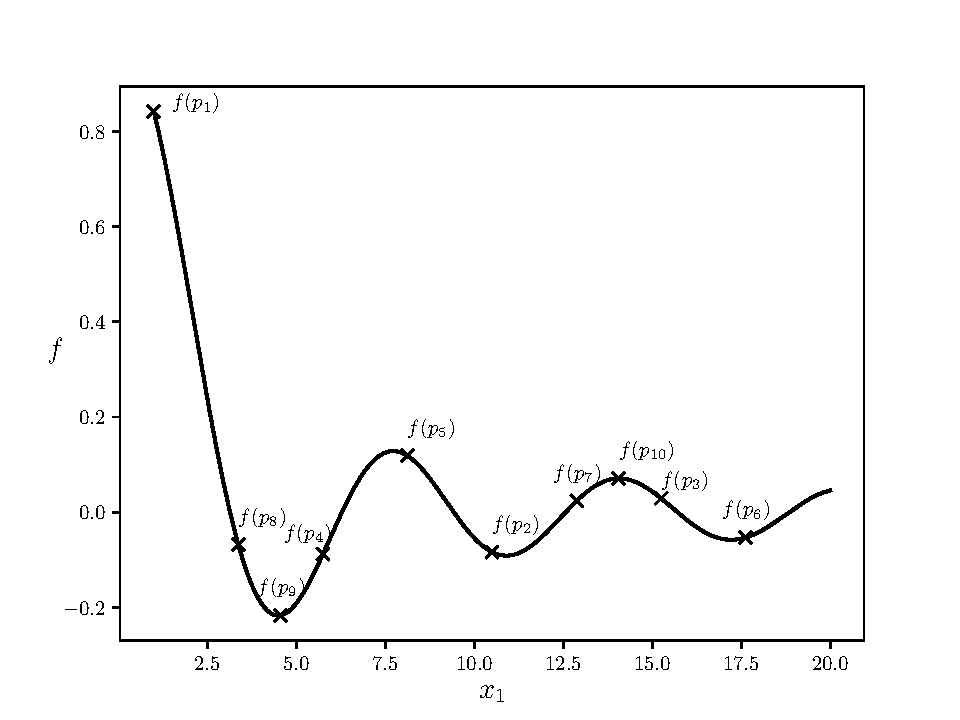
\includegraphics[scale=1.0]{./Fig1.pdf}}
{\caption{Test function give by Equation (\ref{eq:test1}) with 10 Sobol sequenced sampling points} \label{fig:pot1}}
\end{figure}

Observing \Cref{fig:pot1} it is immediately apparent that the set of 10 sampling points alone provides adequate information to deduce that there are at least 3 local minima. Observe that there are at least two other local minima since $ f(p_5) < f(p_2) < f(p_7)$. So at least one local minimum exists in the domain $(p_5, p_7) \subset \mathbb{R}$ since between $p_5$ and $p_2$ we must have, by the mean value theorem (MVT), $\frac{df}{dx} < 0$ for some domain $x \in [p_5, p_2] \subset \mathbb{R}$. Similarly for $x \in [p_2, p_7] \subset \mathbb{R}$ we have by MVT $\frac{df}{dx} > 0$. Since $f$ is a smooth, continuous function for $x \in (0, \infty)$ there must exist at least one stationary point $x  \in (p_5, p_7)  \subset \mathbb{R}$ where $\frac{df}{dx} = 0$. Furthermore we observe $f(p_6) < f(p_3)$ indicating another minimum in the domain $x  \in (p_3, 20] \subset \mathbb{R}$ since the minimum must be either on the boundary or in $x  \in (p_3, 20] \subset \mathbb{R}$ by the same argument as above. % !!TODO: offer a rigorous proof for these statements?!!  

The empirical relation by \citet{Henderson2015} was mainly developed for the purpose of finding the global minimum. Therefore if only $10$ sampling points are available, then in order to find more local minima using the TGO method, it is required to force a lower $k$ value. Alternatively, since $k_c$ is a function of $N$, simply sampling more points is sufficient to find all the local minima using Henderson's formula for this test problem. For example at $N=16$ all 3 local minima are produced by TGO with Henderson's formula. \Cref{fig:min} shows the number of minimisers found at different $k$ values for this example. The maximum minimiser set (other than using every sampling point as a starting point) can be trivially extracted by setting $k=1$ and calculating $|\mathcal{M}^1|$. However, in this Example it leads to more starting points than optimal since at least two minimisers will be in the same convex basin domain and therefore converge to same minimum in the local minimisation step. This results in superfluous function evaluations without extracting more useful information from the objective function. 

This idea drives the motivation behind the following definition.
\begin{definition} \label{def:optpool}
For a given set $\mathcal{P}$ of $N$ sampling points, $k_{opt}$ is any integer $1 \leq k \leq (N -1)$ that will produce the optimal minimiser set $\mathcal{M}^{k_{opt}}$ containing the maximum set of minimisers such that no two starting points extracted from $\mathcal{M}^{k_{opt}}$ will lead to the same minimum in the local optimisation step for some tolerance $\epsilon$. In other words every element contained in $\mathcal{M}^{k_{opt}}$ should lie in a unique locally convex sub-domain.
\end{definition}

Note that for a given $N$, $\mathcal{M}^{k_{opt}}$ might not produce all the true local minima of an objective function. What's important is that, given the information known from the sampling, the maximum number of local minima are found. In addition, no function evaluations are wasted in the local minimisation step which lead to the same minimum.

% !!TODO: THIS IS NOT WRITTEN IN TORN1992 FIND ANOTHER REFERENCE:  This flaw in the TGO algorithm is not unknown, \citet{Torn1992} noted the trade-off between using more local minimisers and the associated computational cost concluding that a larger $k$ value will lead to more function evaluations in the local search step without significant contributions.!!!

\begin{figure}
\centerline{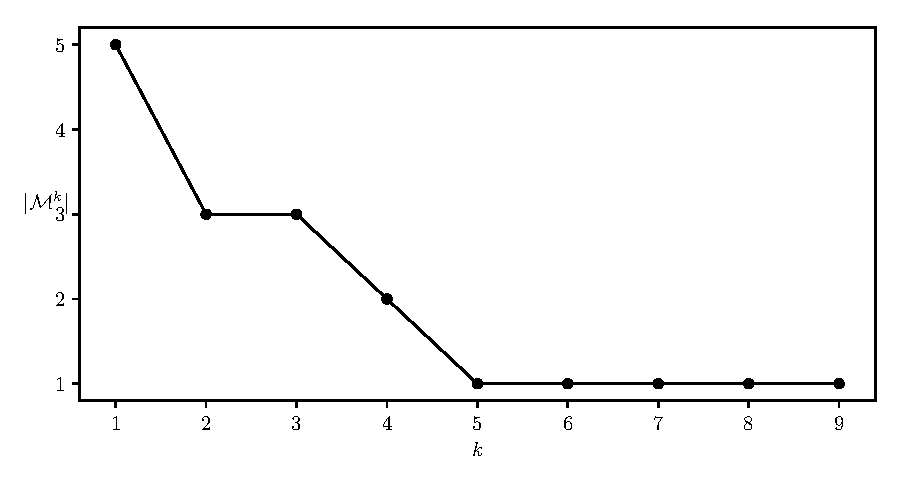
\includegraphics[scale=1.0]{./Fig2.pdf}}
{\caption{Number of minimisers $|\mathcal{M}^k|$ found using the TGO method for different $k$ values at $N = 10$}  \label{fig:min}}
\end{figure}

In Example 1 for $N = 10$ the optimal $k$ values are $k_{opt}=\{2, 3\}$ which will produce 3 minimisers $|\mathcal{M}^2| = |\mathcal{M}^3| = 3$. We will now show that these lower $k$ values carry unexploited information on the best approximate geometry for the objective function. For example in \Cref{fig:mink} we plot the $|\mathcal{M}^k|$ values corresponding to the set $k = \{1, 2, 3, 4, 5, 6, 7, 8, 9, 10\}$ for every sampling point range $N \in [2, 50]$.

\begin{figure} 
\centerline{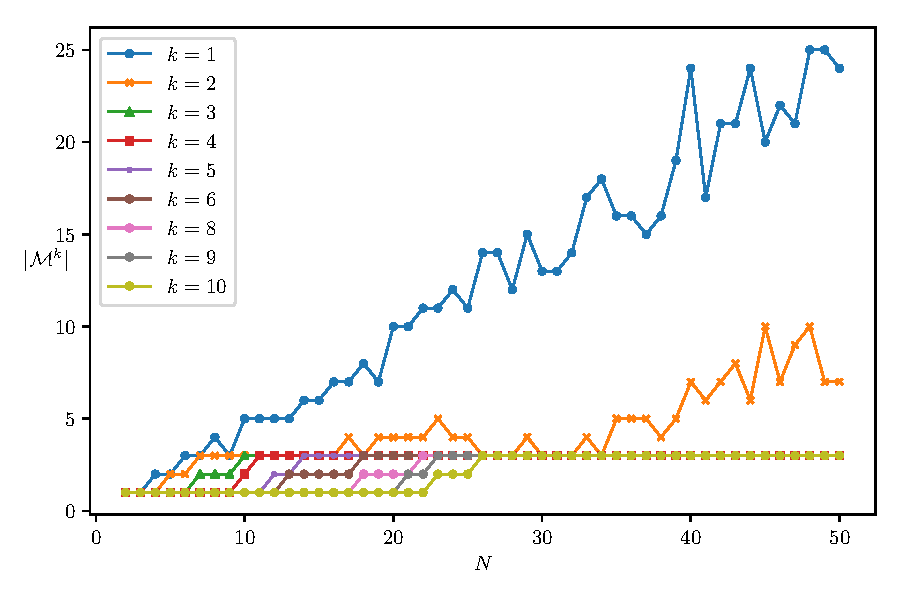
\includegraphics[scale=1.0]{./Fig3.pdf}}
{\caption{Number of minimisers $|\mathcal{M}^k|$ found using the TGO method for the given $k$ values at various sampling points $N$} \label{fig:mink}}
\end{figure}

From \Cref{fig:mink} we notice the special property of $k = 3$ for one dimensional objective functions sampled with the Sobol sequence. 

Firstly, for a lower number of sampling points $N$ it provides a higher number of starting minimisers than $k > 3$. Note that by inspection of Definition \ref{def:tgo3} it can be determined that any $k > 3$ value will always produce an equal or lower number of minimisers than $k = 3$ (this is also true for any $k > i$). When adding columns to a positive row there are only two possibilities: the next sampling point in the row can either have a positive or a negative sign. All other elements in the row have a positive sign by definition (see Definition \ref{def:tgo3}). If the next sampling point in the row has a positive sign then the row will just remain a positive row and the number of minimisers remain the same. If the point is a negative reference point then the row will no longer be a positive row and thus the point is no longer a minimiser, lowering the total.

Secondly it can be observed that $k = 3$ never calculates a number of starting minimisers higher than optimal unlike $k < 3$. Therefore by using $k = 3$ in Example 1 TGO will always find as many minimisers in as few sampling\footnote{not necessarily total function evaluations since starting points closer to the local minima may provide better performance for a given local minimisation routines} function evaluations as possible and furthermore all local minima will be found when $N \ge 10$. It should be noted that the total number of function evaluations depends on the particular local minimisation algorithm used. However, it is apparent that each minimiser starting point is in a unique locally convex domain. It is tempting for an optimisation practitioner to use the size of the set of minimisers $|\mathcal{M}^3|$ as a stopping criterion for iterative sampling $N$ of one dimensional objective functions. The practical usefulness of this idea can be demonstrated with the following example:

\paragraph{Example 2} The following instance of the optimisation problem has 13 local minima in the given domain
\begin{equation} \label{eq:test2}
\underset{x}{\min} ~f(x) = -x \sin(x), ~ x  \in  \Omega = [1, 80]
\end{equation}

From \Cref{fig:mink2} we can deduce that the minimum number of sampling points required for $k = 3$ to find all local minima using the Sobol sequence is $N = 40$, this sampling is shown in \Cref{fig:pot2}.  If  $N < 40$ then there aren't enough sampling points to deduce that there are at least 13 locally convex domains from using the same arguments as in Example 1. Note for example that if we used a sequence that skipped $p_1$ then $N =39$ would be adequate since $l = 1 < p_{32} < p_{33}$. Using our Python implementation of TGO \citep{TGOpy} with $N = 40$ all 13 local minima of the objective function were found in a total of 285 function evaluations. 

An example of a stopping criterion would be to stop sampling if $|\mathcal{M}^3|$ is unchanged after, say, 10 sampling point evaluations. The rate at which the number of elements in $|\mathcal{M}^3|$ grows with increasing $N$ also provides a heuristic for characterising the multimodality and the geometry of the objective function. Objective functions that have a large number of local minima in a small domain (and relatively fewer minima in other larger domains) will have a much smaller growth in $|\mathcal{M}^3|$ for a given low-discrepancy sampling. This idea of continuously classifying and extracting approximate function characteristic information from the sampling points will be formalised and extended to higher dimensions in \Cref{sec:shgo}.


\begin{figure}  \label{fig:mink2}
\centerline{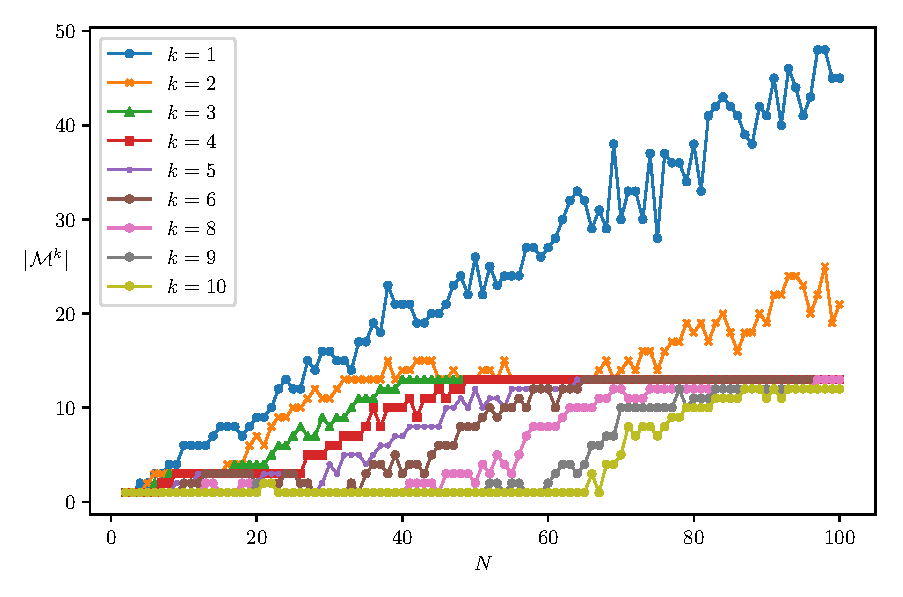
\includegraphics[scale=1.0]{./Fig4.pdf}}
{\caption{Number of minimisers $|\mathcal{M}^k|$ found using the TGO method for the given $k$ values at various sampling points $N$}  \label{fig:mink2}}
\end{figure}

\begin{figure} 
\centerline{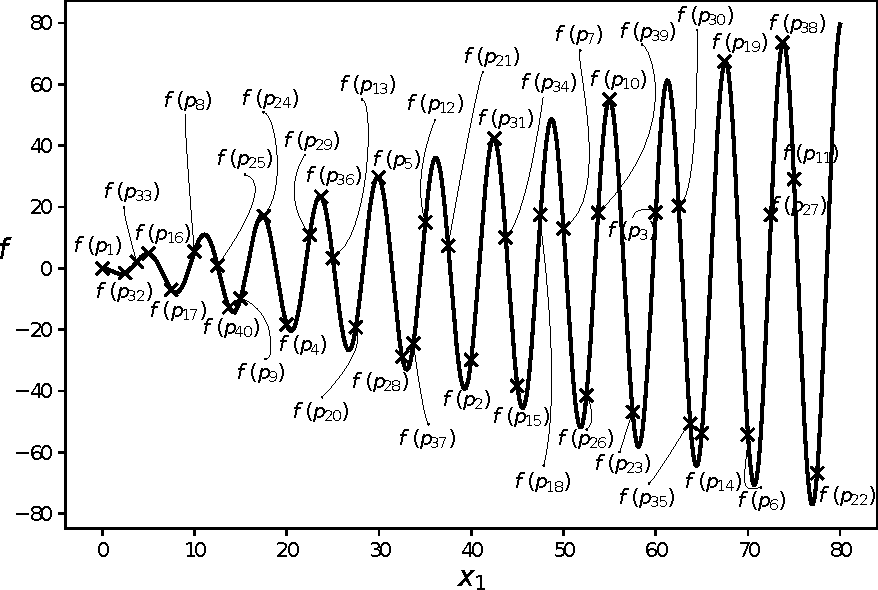
\includegraphics[scale=1.0]{./Fig5.pdf}}
{\caption{Plot of the objective function in Example 2 for $N = 40$ sampling points} \label{fig:pot2}}
\end{figure}

There is a simple reason why the $3$-$t$-matrix has this quality in the first dimension for the optimisation problem given in Equation (\ref{eq:test1}). However, it is not guaranteed that this property holds for any sampling point distribution. In fact it holds true only under the following conditions:
\begin{enumerate}
\item Consider all points in the ordered sampling set from the smallest to greatest $x$ value $\mathcal{P} = \{p_i~|~p_{0}~<~p_{1}~<~p_{2}~\dots~<~p_N-1,~p_{i}~\in~(x_l,~x_u)\}$, excluding the supremum and infimum.
\item For any given point $p_i$ the Euclidean distance between $p_i$ and 2 of its nearest sampling points $p_{i-1} < p_i < p_{i+1}$ should be less than the relative difference between $p_i$ and a fourth point in the sampling sequence $|p_i - p_j|$ where $j \neq {i, i-1, i+1}$.
\end{enumerate}
 
In fact it is easy to prove both that for a locally, strictly convex domain of $f$ the $3-$topograph construction can produce a larger minimiser pool $\mathcal{M}^3$ than optimal. It can also be shown that a construction must exist where the optimal number of minimisers will \it{always} \normalfont be extracted regardless of the sampling distribution. Furthermore it can be shown that at most 3 sampling points within a locally convex domain $x \in [x_l, x_u]$ is required to produce enough information so that only one minimiser in the domain is produced.

\begin{theorem} \label{1d}
There exists a $1$-dimensional sampling sequence such that $k = 3$ will produce a minimiser pool larger than optimal as defined by Definition \ref{def:optpool}.
\end{theorem}

\begin{proof}
Consider a subdomain $x \in [x_l, x_u] \subset \mathbb{R}$ for which $f$ is strictly convex. We define the set of $N$ sampling points $\mathcal{P}$ ordered in such a way that $$\mathcal{P} = \{p_i~|~p_{0}~<~p_{1}~<~p_{2}<~\dots~<~p_{N-1},~p_{i}~\in~(x_l,~x_u)\}$$

Let $\mathcal{F} = \{f_{0},~f_{1},~f_{2},\dots,~f_{N-1}\}$ be set of one-to-one function values corresponding to the points mapped by $f:\mathcal{P} \rightarrow \mathcal{F}$. 

Suppose we have $f_1 < f_0$ and $f_1 < f_2 < f_3, \dots f_{N-1}$.  %, by construction we have  $|p_i - p_j|$
By construction we have  $|p_1 - p_2| < |p_1 - p_3| < |p_1 - p_4| < |p_1 - p_5|$ then by the Definitions \ref{def:tgo1}, \ref{def:tgo2} and \ref{def:tgo3} $p_2$ is a minimiser of the $3-t-$topograph. Suppose we have a sampling distribution such that $|p_2 - p_3| < |p_1 - p_2|, |p_2 - p_4| < |p_1 - p_2|$ and $|p_2 - p_5| < |p_1 - p_2|$ then by the Definitions \ref{def:tgo1}, \ref{def:tgo2} and \ref{def:tgo3} $p_3$ is also a minimiser of the $3-t-$topograph. Therefore more than two minimisers are produced in the same locally convex sub-domain of $[x_l, x_u]$. We have shown that $\mathcal{M}^3$ can produce a minimiser pool larger than optimal which concludes the proof.

\begin{lemma} \label{1dax}
A construction exists that will always produce a minimiser pool larger than optimal as defined by Definition \ref{def:optpool} for any given $1$-dimensional sampling sequence.
\end{lemma}

Now suppose that instead of using only the Euclidean distance metric we also invoke knowledge of the nearest point in all cartesian directions. We use the criterion that a minimiser point $p_i$ is a minimiser iff \normalfont with the ordering constructed in $\mathcal{P}$ and $\mathcal{F}$ we have $f_i < f_{i - 1}$ and $f_i < f_{i + 1}$. With this definition if the point $p_i$ is a minimiser then no other point meets the criterion since by construction of the sampling in the locally convex domain $f_{0} > f_{1} > \dots > f_{i - 1} > f_i$ and $f_{i + 1} < f_{i + 2} < f_{i + 3} < \dots < f_{N-1}$. This proves Lemma \ref{1dax}. 

Finally note that only information from the 3 points in the locally convex sub-domain of $[x_l, x_u]$ and their corresponding function values $f_{i - 1}$, $f_{i}$ and $f_{i + 1}$ are needed to produce a minimiser using this criterion.
\end{proof}

There is an important consequence here for low discrepancy sequences in higher dimensions and for less well behaved objective functions. In both these cases. the topographs connected with the Euclidean distance metrics will discard available information about the local geometry of the objective function surface. This produces larger than optimal minimiser pools leading to very high numbers of function evaluations needed to solve the problem.


%!! TODO: Add visual aide, motivate that this kind of shitty distribution will happen in higher dimensions even for good sequences like Sobol. \\


%Clearly in using the Euclidian distance matrix the information known by contruction (the relative position of the sampling points on the $x$-axis) is lost

%Since the $x$ variable can only vary in one positive or negative direction, however, in higher dimensions...



In the following section we will develop a more efficient algorithm that will make use of this information. SHGO will always produce equivalent results to this algorithm in the one dimensional case.


%\section{Axial}
\section{Axially directed topograph}  \label{sec:atgo}
Based on the observations from \autoref{sec:motivation} we develop an algorithm that, for a given sampling set, always uses the optimal number of starting minimisers as defined for one dimensional objective functions without requiring \it{a-priori} \normalfont specification of the $k$ parameter. Here a new graph structure is proposed and attempts are made to directly extend the idea to higher dimensions by connecting every vertex to the nearest vertex in every cartesian axis direction. In Theorem \ref{theorem:iff1} we show that the one dimensional properties of this algorithm does not extend to higher dimensions which finally leads us to the built up complexes in \autoref{sec:shgo}. The main conclusion of this section is that simpler graph structures cannot be used to find locally convex sub-domains of a function in the same way that was accomplished in \autoref{sec:motivation}.

The algorithm proceeds in the same way as TGO described in \autoref{sec:TGO} except for step 2 where a new structure described in Section 4.1 replaces the topograph. 


\subsection{Axially directed topograph}
Let $\mathcal{F}$ be the set of scalar outputs mapped by the objective function $f:\mathcal{P} \rightarrow \mathcal{F}$ for a given sampling set $\mathcal{P} \subseteq \Omega \subseteq \mathbb{R}^n$. The scalar elements $f_i \in \mathcal{F}$ have one-to-one correspondence with the vector elements $\bold{p}^i \in \mathcal{P}$ where the integer $i \in \{1, 2, 3, \dots, N\}$ indicates the sampling point index. The vector $\bold{p}^i$ in turn has dimensional elements $x_j^{i}$ where the integer $j \in \{1, 2, 3, \dots, n\}$ indicates the dimension of the scalar value  $\forall i (x^{i}_1,~x^{i}_2,~x^{i}_3,~\dots,~x^{i}_n) \in \bold{p}^i$. 

We wish to construct a graph that is ordered along the coordinate axes, this is done by formally defining the following related partially ordered sets.

\begin{definition} \label{def:indexset}
Given a finite structured set of $N$ feasible ordered sampling points $\mathcal{P} = (\bold{p}^1, \bold{p}^2, \dots, \bold{p}^N )$ with its corresponding objective function outputs $\mathcal{F} = (f^1, f^2, \dots, f^N )  $, the index set of $\mathcal{P}$ is given as the ordered set $\mathcal{I} = ( i = \{1, 2, 3, \dots, N\}, \leq) $
%Given a finite set of $N$ feasible sampling points $P_1, P_2, \dots, P_N \in \mathcal{P}$ with its corresponding objective function outputs $ \mathcal{F}$, the index set of $\mathcal{P}$ is given as the ordered set $\mathcal{I}= ( i = \{1, 2, 3, \dots, N\}, \leq) $.
\end{definition}
Note that the initial ordering of the index set is arbitrary, what's important is that an ordered index set is defined. This ordering will allow us to keep track of any vertex in the graph to its corresponding sampling point in $\mathcal{P}$ so that the corresponding objective function only needs to be evaluated once. Herein the order is taken as the order that is generated by the Sobol sequence. 

\begin{definition}  \label{def:atgo2}
Given a set of feasible sampling points $\mathcal{P} \subseteq \Omega \subseteq \mathbb{R}^n$ define $X_j$ for every dimension $ j \in \{1, 2, 3, \dots, n\}$  as the partially ordered set $X_j = \{\bold{p}^i~|~\forall i (x^i_j < x^{i + 1}_j) \}$.
%Given a set of feasible sampling points $\mathcal{P} \subseteq \Omega \subseteq \mathbb{R}^n$ define $X^j$ for every dimension $ j \in \{1, 2, 3, \dots, n\}$  as the set $\textrm{\normalfont poset} X^j = (\bold{x}_0, \bold{x}_1, \dots, \bold{x}_N)$ where the vectors $\bold{x}_k$ are defined as $\forall j( \{(\bold{x}_0, \bold{x}_1, \dots, \bold{x}_N)~|~(x_{0, j} \le x_{1, j} \le \dots \le x_{k, j}),  x_{k, j} \in P_i \in \mathcal{P} \})$ with $ k \in \{1, 2, 3, \dots, N\}$.
\end{definition}

%!!!We don't need to define $\mathcal{I}$ using the other definitions!!!
%\begin{definition}
%For every dimension $j$, $\mathcal{I}_j$ is the ordered set of integers such the position of the elements $X_j$ correspond to the original index sampling of $ \mathcal{P}$. $\mathcal{I}_j = \{i~|~\forall i (x^i_j < x^{i + 1}_j) \}$  %$\{(i, i, \dots, i) | i \in \mathcal{I} \}$\
%\end{definition}

The definition is demonstrated with the following numerical example:

\paragraph{Example 3} Given set of the first 5 points in the 2-dimensional Sobol sequence bounded by the 2-cube: $$\mathcal{P}~=~\left((0,~0),~(0.5,~0.5),~(0.75,~0.25),~(0.25,~0.75),~(0.375,~0.375)~\right)~\subseteq~[0,~1]~\times~[0,~1] \subseteq~\mathbb{R}^2$$ let $f(x) = x_1^2 + x_2^2$ so that
$$\mathcal{F} = (0,~0.5,~0.625,~0.625,~0.28125)$$
then 
$$X_1 = ((0,~0), (0.25,~0.75), (0.375,~0.375), (0.5,~0.5), (0.75,~0.25))$$
and 
$$X_2 = ((0,~0), (0.75,~0.25), (0.375,~0.375), (0.5,~0.5), (0.25,~0.75))$$
The corresponding index sets are $\mathcal{I}_1 = (1, 4, 5, 2, 3)$ and $\mathcal{I}_2 = (1, 3, 5, 2, 4)$.  

\begin{definition} \label{def:atgo3}
For every dimension $j$, $\mathcal{F}_j$ is the partially ordered set such that the position of the elements $X_j$ correspond to the original index sampling of $ \mathcal{P}$, $\mathcal{F}_j = \{f^{i, k}_j~|~\forall i (x^i_j < x^{i + 1}_j), f^{i, k}_j = f_k \in \mathcal{F}, k \subseteq  \mathcal{I} \}$ 
\end{definition}
%!!! $f^{i, k}_j = f_k \in \mathcal{F} \rightarrow$  This term needs to be more clear !!!
That is the first superscript $i$ of the elements $f^{i, k}$ indicate the ordering in $\mathcal{F}_j$, while the second superscript $k$ indicates the corresponding scalar value of $f^{i, k}$ in $ \mathcal{F}$. Ordering the example we have
$\mathcal{F}_1 = (0,~0.625,~0.28125,~0.5,~0.625)$ and  $\mathcal{F}_2 = (0,~0.625,~0.28125,~0.5,~0.625)$.


\begin{definition}
For every dimension $j$, define the partially ordered sets of cardinality $N$ such that $\mathcal{F}^+_j = \{{f}^{i, k}_j - {f}^{i - 1, k}_j~|~\forall i (x^i_j < x^{i + 1}_j), f^{i, k}_j = f_k \in \mathcal{F}, i = \{1, 2, \dots, N , k \subset \mathcal{I} \} \}$ and $\mathcal{F}^-_j = \{{f}^{i, k}_j - {f}^{i + 1, k}_j ~|~\forall i (x^i_j < x^{i + 1}_j), f^{i, k}_j = f_k \in \mathcal{F}, i = \{0, 1, \dots, N - 1 \}, k \subset \mathcal{I} \}$ \label{def:atgo4}
\end{definition} 
These sets are essentially objective function differences between the sampling points along each dimensional Cartesesian axis. Continuing from the numerical example we have
\begin{align} \nonumber
\mathcal{F}_1^+ =&~ (~0.625, -0.34375, ~0.21875, ~0.125) \\  \nonumber
\mathcal{F}_2^+ =&~ (-0.625, ~0.34375, -0.21875, -0.125) \\  \nonumber
\mathcal{F}_1^- =&~ (~0.625, -0.34375,  ~0.21875, ~0.125) \\  \nonumber
\mathcal{F}_2^- =&~ (-0.625, ~0.34375, -0.21875, -0.125) 
\end{align}

We denote the elements as $ f_j^{+i, k} \in \mathcal{F}_j^+$ and $ f_j^{-i, k} \in \mathcal{F}_j^-$ for every dimension $ j \in \{1, 2, 3, \dots, n\}$, cartesian ordering $i \subseteq \mathcal{I}$ and corresponding sampling point $k \in \mathcal{I}$.  The usefulness of these abstract constructions is apparent in the following definition.

\begin{definition} \label{def:carpool}
For a given sampling set $\mathcal{P}$. The minimiser pool $\mathcal{M}$ is defined as 
$$\mathcal{M} =\mathcal{M}_c  \cup \mathcal{M}_{lb}   \cup \mathcal{M}_{ub} $$
where

$\mathcal{M}_c = \left\{ \bold{p}^i~|~\forall j \left( (f_j^{+i} > 0 )	\land (f_j^{-(i+1)} > 0) \right), i = \{1, 2, 3, \dots, N - 1\} \right\}$

$\mathcal{M}_{lb} = \left\{ \bold{p}^i~|~\forall j \left(f_j^{-i} < 0\right), i = \{0\} \right\} $

$\mathcal{M}_{ub}=  \left\{ \bold{p}^i~|~\forall j \left(f_j^{+i} < 0 \right), i = \{N\} \right\} $

%$\mathcal{M_1} = \left{ \bold{p}^i~|~\forall j \left( (f_j^{+i} > 0 )	\land (f_j^{-(i+1)} > 0) \right), i = \{2, 3, \dots, N - 1\}\right}$ $ \cup  \left{ \bold{p}^i~|~\forall j \left(f_j^{-i} < 0\right), i = \{0\}\right} \cup  \left{ \bold{p}^i~|~\forall j \left(f_j^{+i} < 0 \right), i = \{N\}\right} $
\end{definition}

That is, we simply check the finite difference between sampling points in every cartesian direction. In addition we check if the sampling points on the boundaries are minimisers.

\begin{theorem} \label{theorem:iff1}
The minimiser pool $\mathcal{M}$ from \autoref{def:carpool} always produces a set that is either smaller than or equal to the optimum minimiser pool as defined by \autoref{def:optpool} iff $j = 1$.
\end{theorem}
\begin{proof}
The proof for $j = 1$ follows the same argument from \autoref{sec:motivation}. By Definition \ref{def:indexset}, \ref{def:atgo2} and \ref{def:atgo3} we have the ordering constructed as $\mathcal{P}$ and $\mathcal{F}_1$. If a given point $\bold{p}^i$ is a minimiser with $f_1^{+i} > 0$ and $f_1^{-i} > 0$, then we have by Definition \ref{def:atgo4} $f^i < f^{i - 1}$ and $f^i < f^{i + 1}$, conversely if a given point $\bold{p}^i$ is not a minimiser then either $f_1^{+i} < 0$ or $f_1^{-i} > 0$ so that regardless of the sampling method used and the Euclidean distance between points a minimiser will never be generated for any point that has $\left((f^i > f^{i - 1}) \land (f^i > f^{i + 1} )\right) \lor \left(( f^i < f^{i - 1}) \land (f^i < f^{i + 1} ) \right)$.

If $j > 1$ we have no such guarantee for a higher dimensional locally convex domain. As a counter example consider the set of points $$\mathcal{P} = \left( (0,~0), (0.25,~0.25), (0.75,~0.125), (0.125,~0.75)\right)$$ on the same function as above, the minimiser set produced is $\mathcal{M} = \{(0,~0),~(0.25,~0.25)\}$ which is clearly larger than optimal and will produce the same local minimum. % TODO: Show calculations?
\end{proof}

This unsatisfactory result for higher dimensions could still potentially show good performance for more regular spaced sampling such as grids, however, as we will see in the next section the SHGO algorithm can guarantee that the optimal minimiser set will be produced for any dimension. 
%!! We stated if and only if so also provide proof that for $j>1$!!!
%!! TODO: Provide a visual aid for this proof? !!

%!!TODO: Can construct arrays/matrices, use boolean values to give formula for calculating M!!

\subsection{Implementation}
Algorithm \ref{alg:atgo} provides a high-level overview of the ATGO algorithm. A Python implementation of this algorithm can be found in \cite{SHGOpy}. 

\begin{algorithm}
\caption{ATGO algorithm}
\label{alg:atgo}
\begin{algorithmic}[1]
\Procedure{Initialisation}{}
\State \bf{Input} \normalfont an objective function $f$, constraint functions $\mathbf{g}$ and variable bounds and $[\mathbf{l}, \mathbf{u}]^n$.
\State \bf{Input} \normalfont $N$ initial sampling points.
\State Define a sampling sequence that generates a set $\mathcal{X}$ of sampling points in the unit hypercube space $[\mathbf{0}, \mathbf{1}]^n$
\EndProcedure
\Procedure{Initial sampling}{}
\State $\mathcal{P} = \emptyset$
\While{$|\mathcal{P}|$ $<$ $N$}
\State Generate $N - |\mathcal{P}|$ sequential sampling points $\mathcal{X} \subset \mathbb{R}^n$
\State Stretch $\mathcal{X}$ over the lower and upper bounds $[\mathbf{l}, \mathbf{u}]^n$
\State  $\mathcal{P} = \{\mathcal{X}_i ~|~ \mathbf{g}(\mathcal{X}_i) \geq 0, \forall \mathcal{X}_i \in \mathcal{X}\} \cup\mathcal{P}$ 
\Comment (Find $\mathcal{P}$ in the feasible subset $\Omega$ by discarding any points mapped outside the linear constraints $g$ and adding to the current set of $\mathcal{P}$.)
\State Set $\mathcal{X} = \emptyset$
\EndWhile
\State Find $\mathcal{F}$ from the objective function $f: \mathcal{P} \rightarrow \mathcal{F}$
\EndProcedure
\Procedure{Construct $\mathcal{M}$}{}
%\State Calculate $\mathcal{F}^+_j$, $\mathcal{F}^-_j$ and $\mathcal{M}$ using Definitions \autoref{def:indexset} through \autoref{def:carpool}.
\State Calculate $\mathcal{M}$ from the sets $\mathcal{P}$ and $\mathcal{F}$ using Definitions \ref{def:atgo2} through \ref{def:carpool}.
\EndProcedure
\Procedure{Local minimisation}{}
\State Calculate the approximate local minima of $f$ using a local minimisation routine with the elements of $\mathcal{M}$ as starting points.
\Comment These local minimisations can be performed in parallel.
\EndProcedure
\Procedure{Process return objects}{}
\State Order the final outputs of the minima of $f$ found in the local minimisation step to find the approximate global minimum.
\EndProcedure \\
\Return the approximate global minimum and a list of all the minima found in the local minimisation step.
\end{algorithmic}
\end{algorithm} 


%\subsection{Applications in one dimension}\label{sec:atgo_a}
%Consider again the objective function given in Example 1.

%!! NOTE: I believe including figures here would be too much, otherwise we can have a figure showing the minimiser pool growth.

%\subsection{Applications in two dimensions}\label{sec:atgo_a}
%!! NOTE:  (Show failure in example paraboloidic function, Sobol points too far on the graph are connected providing visual clues as to why it fails, we can recommend experiments with other low discrepancy sequences or regularly spaced grids). If we do this it will be at least 2+ more pages though.



%\section{shgo}
\chapter{Simplicial Homology Global Optimisation}  \label{sec:shgo}
\section{Overview}
The SHGO method strongly relies on constructing a simplicial complex using the sampled points of an objective function $f$ as vertices. From this construction of the complex $\mathcal{H}$ we use the resulting directed subgraph which contains the set of all $1-$chains from the elements of $\mathcal{H}^1 \in \mathcal{H}$ to find minimiser pools using definitions similar to the methods demonstrated in the previous sections. This is accomplished by the application of Sperner's lemma \cite{Sperner1928} allowing us to approximate the domains of stationary points for any objective function in the feasible search space $\Omega$. 

We prove that, if provided with an adequate sampling set, the construction of $\mathcal{H}$ will produce the same homology groups. We use this result to show that for the given sampling set of vertices $\mathcal{H}^0 \in \mathcal{H}$ we always extract the optimal minimiser pool similar to the one-dimensional case described in \autoref{sec:motivation}, but extended to higher dimensions. 

The algorithm itself consists of four steps which will described in detail:
\begin{enumerate}
\item Uniform sampling point generation of N vertices in the search space within the bounded and constrained subspace of $\Omega$ from which the $0-$chains of $\mathcal{H}^0$ are constructed.
\item Construction of the directed simplicial complex $\mathcal{H}$ by triangulation of the vertices.
\item Construction of the minimiser pool $\mathcal{M} \subset \mathcal{H}^0$ by repeated application of Sperner's lemma.% and the Lefschetz Fixed Point Theorem.
\item Local minimisation using the starting points defined in $\mathcal{M}$.
\end{enumerate}

We will start by formally defining the construction of $\mathcal{H}$ from a given set of feasible sampling points $\mathcal{P}$ and proving its properties. %In this paper we will consider only a search space defined by a bounded hyperrectangle $\Omega \subseteq  [l, u]^n\subseteq\mathbb{R}^n$ with $\mathcal{P} \in \Omega$. It is easily extended to optimisation problems with simple linear constrains in $\mathbf{g}$ since the resulting space is compact and convex, however, care must taken if $\mathbf{g}$ contains non-trivial, non-linear constraints !!TODO: CITE NEW SECTION PROOF. In the practical implementation of the algorithm non-linear constraints can be defined, however, the properties defined here are not guaranteed.


\section{Directed simplicial complex approximation of the objective function}
Consider again the general objective function mapping in the continuous domain $f : \mathbb{R}^n \rightarrow \mathbb{R}$. The purpose of this section is describe a discrete mapping $h: \mathcal{P}\rightarrow \mathcal{H}$ to provide a simplicial approximation for the surface of $f$. To guide the reader the methods will be demonstrated on the simple 2-dimensional optimisation problem defined in Example 4. The use of a 2-dimensional surface allows a demonstration of the techniques while the abstractions defined are readily extended to higher dimensions. 

We start by formally defining the set of vertices from which $0-$chains of the simplicial complex are built and the of edges from which the $1-$chains of $\mathcal{H}$ are built.

\begin{definition} \label{def:h0}
Let  $\mathcal{X}$ be the set of sampling points generated by a sampling sequence in the bounded hyperrectangle $[\mathbf{l}, \mathbf{u}]^n$. The set $\mathcal{P} = \{\mathbf{x} \in \mathcal{X}~|~\mathbf{g}(\mathbf{x}) \geq 0 \}$ is a set of points within the feasible set $\Omega$ .
\end{definition}

\begin{definition} \label{def:h0.5}
For an objective function $f$, $\mathcal{F}$ is the set of scalar outputs mapped by the objective function $f:\mathcal{P} \rightarrow \mathcal{F}$ for a given sampling set $\mathcal{P} \subseteq \Omega \subseteq \mathbb{R}^n$.
\end{definition}

\begin{definition} \label{def:h1}
Let $\mathcal{H}$ be a directed simplicial complex. Then $\mathcal{H}^0 := \mathcal{P}$ is the set of all vertices of $\mathcal{H}$ .
\end{definition}

\begin{definition} \label{def:h2}
For a given set of vertices $\mathcal{H}^0$, the simplicial complex $\mathcal{H}$ is constructed by a triangulation connecting every vertex in $\mathcal{H}^0$. The triangulation supplies a set of undirected edges $E$.
\end{definition}

%\begin{definition} 
%For a given sampling set $\mathcal{P}$. The minimiser pool $\mathcal{M}$ is defined as 
%$\mathcal{M} = \{ \bold{p}^i~|~\forall j(f_j^{+i} > 0 	\land f_j^{-i} > 0), i = \{2, 3, \dots, N - 1\}\} \cup  \{ \bold{p}^i~|~\forall j(f_j^{-i} < 0), i = \{0\}\} \cup  \{ \bold{p}^i~|~\forall j(f_j^{+i} < 0), i = \{N\}\} $
%\end{definition}

\begin{definition} \label{def:h3}
The set $\mathcal{H}^1$ is constructed by directing every edge in $E$. A vertex $v_i \in \mathcal{H}^0$ is the connected to another vertex $v_j$ by an edge contained in $E$. The edge is directed as $\overline{v_i v_j}$ from $v_i$ to $v_j$ iff $f(v_i) < f(v_j)$ so that $\partial \left( \overline{v_i v_j} \right) = v_j - v_i$. Similarly an edge is directed as $\overline{v_j v_i}$ from $v_j$ to $v_i$ iff $f(v_i) > f(v_j)$ so that $\partial \left( \overline{v_j v_i} \right) = v_i - v_j$.
\end{definition}

For practical computational reasons we must also consider the case where $f(v_i) = f(v_j)$. If neither $v_i$ or $v_j$ is already a minimiser we will make use of rule that the incidence direction of the connecting edge is always directed towards the vertex that was generated earliest by the sampling point sequence. If $v_i$ is not connected to another vertex $v_k$ then we leave the notation $\overline{v_i v_k}$ undefined and let $\partial \left(\overline{v_i v_k}\right) = 0$. We let the higher dimensional simplices of $\mathcal{H}^k, k = 2, 3, \dots n + 1$ be directed in any arbitrary direction which completes the construction of the complex $h: \mathcal{P}\rightarrow \mathcal{H}$. We can now use $\mathcal{H}$ to find the minimiser pool for the local minimisation starting points used by the algorithm:

\begin{definition} \label{def:h4}
A vertex $v_i$ is a minimiser iff every edge connected to $v_i$ is directed away from $v_i$, that is $\partial \left( \overline{v_i v_j} \right) = (v_{j \neq i} - v_i) \lor 0~ \forall v_{j \neq i} \in \mathcal{H}^0$. The minimiser pool $\mathcal{M}$ is the set of all minimisers.
\end{definition}
%!!TODO: Be more explicit in defining $h$ precisely


We will also make extensive use of star notation \cite{Hatcher2011, Henle1979}:
\begin{definition} \label{def:h5}
The star of a vertex $v_i$, written $\textrm{st}\left( v_i \right)$, is the set of points $Q$ such that every simplex containing $Q$ contains $v_i$. \
\end{definition}
The $k-$chain $C(\mathcal{H}^k), k = n + 1$ of simplices in $\textrm{st}\left( v_i \right)$ forms a boundary cycle $\partial(C(\mathcal{H}^{n + 1}))$ with $\partial\left(\partial(C(\mathcal{H}^{n + 1}))\right) = \emptyset$. The faces of $\partial(\mathcal{H}^{n + 1})$ are the bounds of the domain defined by $\textrm{st}\left( v_i \right)$.

A visual demonstration of these constructions and notations is provided in the following numerical example:

\paragraph{Example 4} The Ursem01 function for two dimensions is defined as follows \cite{Gavana2016}
\begin{equation*}
\min f(\bold{x}) =  \displaystyle - \sin{\left(2 x_1  - 0.5 \pi \right) - 3 \cos{\left(x_2\right)}} - 0.5 x_1 , ~ x \in \Omega =  [0, 9] \times [-2.5, 2.5] 
\end{equation*}
\autoref{fig:ursem} provides a 3 dimensional plot of this function. The function has three local minima within the domain $\bold{x} \in [0, 9] \times [-2.5, 2.5]$.

\begin{figure} 
\centerline{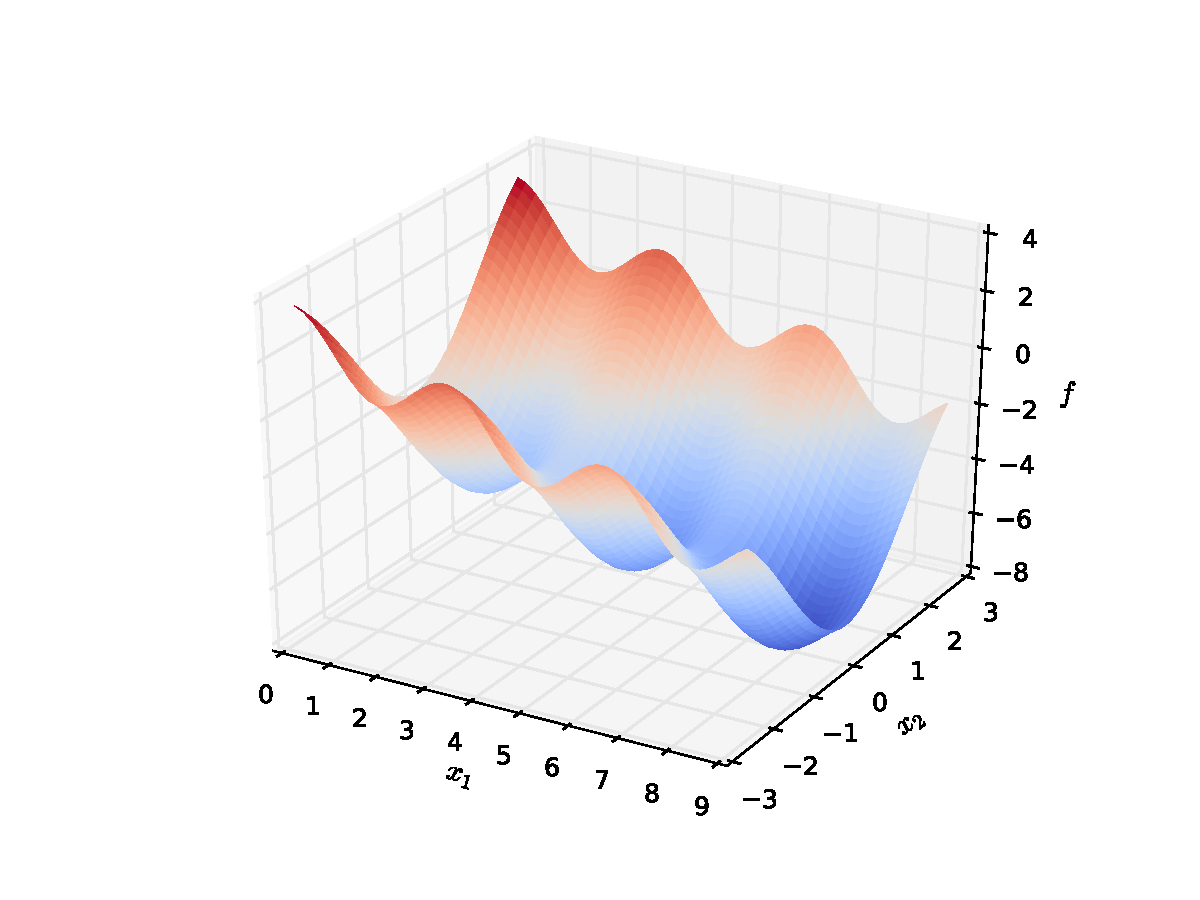
\includegraphics[scale=0.7]{./Fig6.pdf}}
{\caption{A 3-dimensional surface plot of the optimisation test function given in Example 4 $ f(\bold{x}) =  \displaystyle - \sin{\left(2 x_1  - 0.5 \pi \right) - 3 \cos{\left(x_2\right)}} - 0.5 x_1$ for the domain $\bold{x} \in \Omega = [0, 9] \times [-2.5, 2.5] $} \label{fig:ursem}}
\end{figure}

We use a set $\mathcal{P}$ of 15 sampling points from the 2-dimensional Sobol sequence. First map out the objective function values:
\begin{equation} \label{eq:ursemmap}
f:
\begin{bmatrix} [l]
v_{0} = (0.0, -2.5) \\
v_{1} = (4.6, 0.0) \\
v_{2} = (6.9, -1.25) \\
v_{3} = (2.3, 1.25) \\
v_{4} = (3.45, -0.625) \\
v_{5} = (8.05, 1.875) \\
v_{6} = (5.75, -1.875) \\
v_{7} = (1.15, 0.625) \\
v_{8} = (1.725, -0.9375) \\
v_{9} = (6.325, 1.5625) \\
v_{10} = (8.625, -2.1875) \\
v_{11} = (4.025, 0.3125) \\
v_{12} = (2.875, -1.5625) \\
v_{13} = (7.475, 0.9375) \\
v_{14} = (5.175, -0.3125)  
\end{bmatrix}
\rightarrow
\begin{bmatrix} [l]
f_{0} = 3.403\\
f_{1} = -6.275\\
f_{2} = -4.0651\\
f_{3} = -2.208\\
f_{4} = -3.3429\\
f_{5} = -4.051\\
f_{6} = -1.493\\
f_{7} = -3.674\\
f_{8} = -3.591\\
f_{9} = -2.191\\
f_{10} = -2.606\\
f_{11} = -5.062\\
f_{12} = -0.601\\
f_{13} = -6.239\\
f_{14} = -6.044
\end{bmatrix}
\end{equation}

From \autoref{def:h1} we find $\mathcal{H}^0$ from $\mathcal{P}$. Next we use Delaunay triangulation to find a set of connected edges according to \autoref{def:h2}. Any triangulation scheme resulting in a simplicial complex can be used. Next the edges are directed from the calculated values of $\mathcal{F}$ using \autoref{def:h3}. Finally from \autoref{def:h4} we find the minimiser set $\mathcal{M} = \{v_{1}, v_{7}, v_{13}\}$. The resulting structure is shown in \autoref{fig:alp5}. Also shown in \autoref{fig:alp5} is the domain of $\textrm{st}\left( v_1 \right)$ for a visual description of \autoref{def:h5}. Next we increase the sampling size to $N = 150$ points and repeat the procedure. The resulting complex is shown in \autoref{fig:alp100}. Notice that while the minimiser vertices have changed (now closer to the true continuous local minima), the cardinality of the minimiser pool $|\mathcal{M}|$ remains unchanged. That is, given an adequate number sampling points $|\mathcal{M}|$ will cease to grow with increasing $N$, providing a heuristic for the number of sampling points needed to approximately map all minima of an objective function. This useful property of the SHGO algorithm is proven formally in \autoref{sec:invariance}. 

\begin{figure} 
\centerline{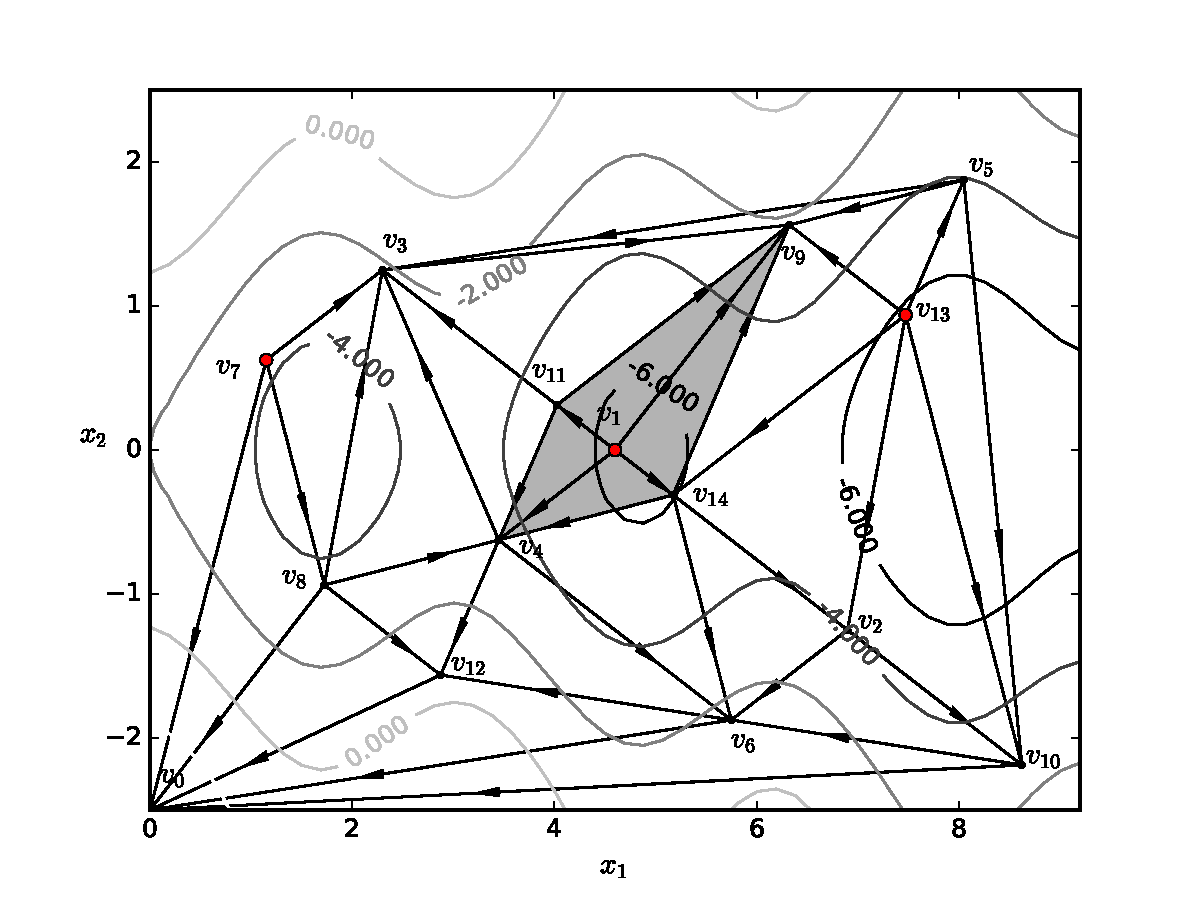
\includegraphics[scale=0.65]{./Fig7.pdf}}
{\caption{A directed complex $\mathcal{H}$ forming a simplicial approximation for an objective function. There are three minimiser vertices $v_1$, $v_7$ and $v_{13}$ shown by the big red dots. The area shaded in grey represents the domain defined by $\textrm{st}\left( v_1 \right)$} \label{fig:alp5}}
\end{figure}

\begin{figure} 
\centerline{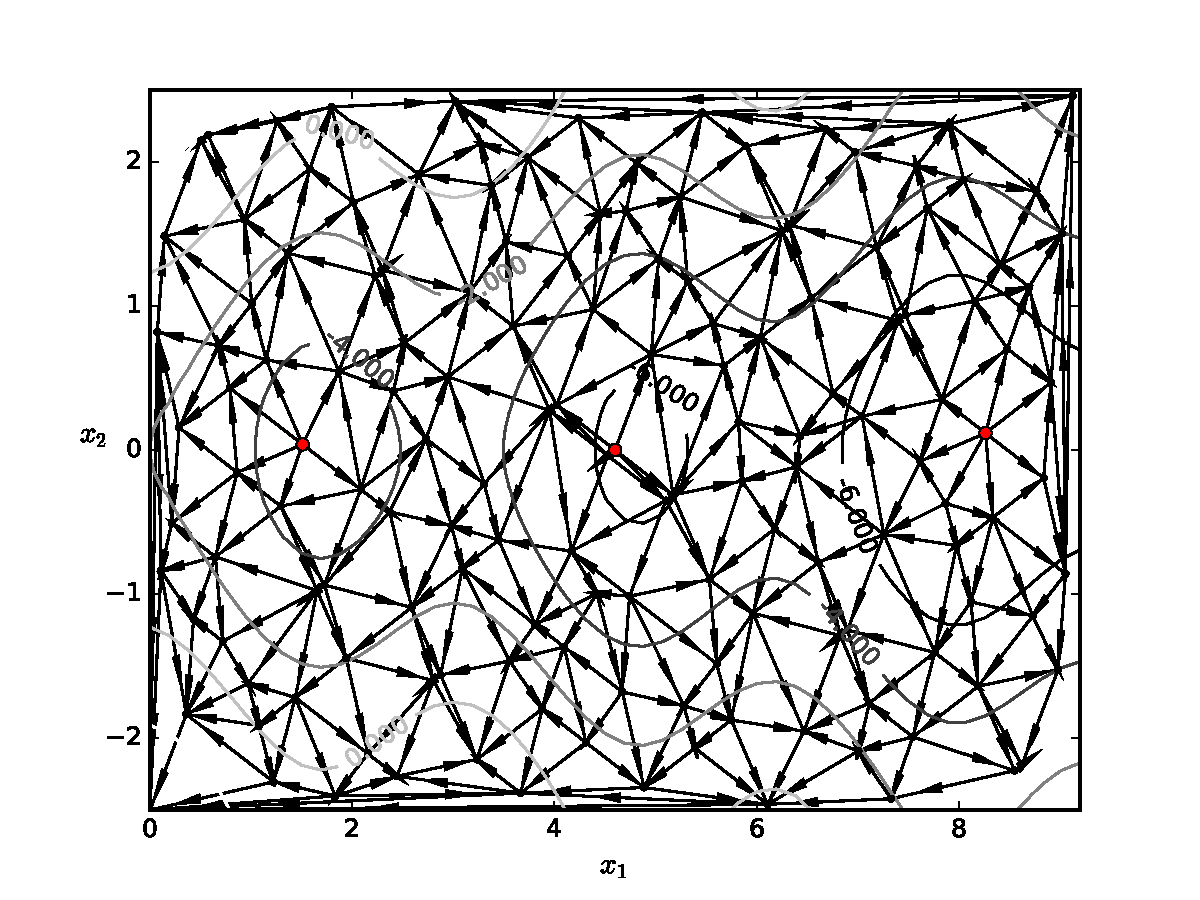
\includegraphics[scale=0.65]{./Fig8.pdf}}
{\caption{A directed complex $\mathcal{H}$ forming a simplicial approximation for an objective function with 150 vertices. There are three minimiser vertices given by the big red dots} \label{fig:alp100}}
\end{figure}

\section{Guarantee of stationary points in sub-domains near minimiser points}
This section is devoted to proving the following theorem:
\begin{theorem} \label{theor:stat}
%Given a minimiser $v_i \in \mathcal{M} \subseteq \mathcal{H}^0$ on the surface of a continuous, Lipschitz smooth objective function $f$ with a compact bounded domain in $\mathbb{R}^n$ and range $\mathbb{R}$. For any $n-$dimensional $k-$chain $C(\mathcal{H}^k), k = n + 1$ with subset of edges $E \subseteq \{C(\mathcal{H}^k), k = n + 1\}\subset \mathcal{H}^1$. If $v_i$ has incidence on a set of edges $E$, then the chain of simplices containing $E$ defines a $k-$chain $C(\mathcal{D}^k)$, $\mathcal{D}^k \subseteq \mathcal{H}^k$, $k=n+1$ near $v_i$ with every vertex in $C(\mathcal{D}^k)$ connected to $v_i$. There exists at least one stationary point of $f$ within the domain defined by the boundary cycle $\partial(\mathcal{D}^{n + 1})$.
Given a minimiser $v_i \in \mathcal{M} \subseteq \mathcal{H}^0$ on the surface of a continuous, Lipschitz smooth objective function $f$ with a compact bounded domain in $\mathbb{R}^n$ and range $\mathbb{R}$, there exists at least one stationary point of $f$ within the domain defined by $\textrm{st}\left( v_i \right)$.
\end{theorem}

\begin{proof}
Our strategy relies on finding a simplex with a Sperner labelling where each label represents a different $n + 1$ label in every vector direction of the gradient vector field $\nabla f$ of $f$ where of the $n + 1$ Cartesian directions we require only a vector pointing towards a section defined by $n + 1$ hyperplane cuts, the remainder of the proof then proceeds as usual for Brouwer's fixed point theorem \cite{Brouwer1911} found in for example \citet[p. 40]{Henle1979} utilising Sperner's lemma.

\begin{theorem} (Sperner's lemma \citep{Sperner1928}) Every Sperner labelling of a triangulation of a n-dimensional simplex contains a cell labelled with a complete set of labels:  {1,2, \dots, n+1}.
\end{theorem}

Start with the observation that for any minimiser $v_i \in \mathcal{M} \subseteq \mathcal{H}^0$ we have by construction that for any vertex $v_j$ with incidence on a connecting edge $\overline{v_i v_j}$ that $f(v_i) < f(v_j)$, so by the MVT there is at least one point on $\overline{v_i v_j}$ where $\nabla f$ points towards a Cartesian direction in a section that can receive a unique Sperner label. If we have $n+1$ vertices with incidence on an edge $ \overline{v_i v_j}\subseteq \mathcal{H}^1$ in every required Cartesian direction then we have a simplex within $\textrm{st}\left( v_i \right)$ with a Sperner labelling. 

In the case where we do not have $n+1$ vertices in every required section then by construction there is no vertex between $v_i$ and the boundary of $f$ defined by $\Omega$ in the required section. In the case where the constraint is not active and there exists at least one point $v_k$ boundary where $\nabla f$ does not point towards the boundary and by the MVT $v_k$ can receive a unique Sperner label from which we can construct a simplex within $\textrm{st}\left( v_i \right)$ with Sperner labelling.

Following the combinatorial version of Brouwer's fixed point theorem \cite{Henle1979} since $\nabla f$ is continuous and the domain $\textrm{st}\left( v_i \right)$ is compact we can produce a sequence of complete triangulations with arbitrarily small size in which the size of the simplices decreases toward zero. This sequence produces a sequence of vertices with gradients $\nabla f(V)$ pointing in every $n+1$ direction. By continuity there is a vector $\nabla f (\mathbf{X})$ near the sequences, since the zero vector is the only vector pointing in all $n+1$ directions we have a point $\mathbf{X}$ bounded by the domain defined by $\textrm{st}\left( v_i \right)$ where $\nabla f (\mathbf{X}) = \bar{0}$.
In the case where the constraint is active a local minimum lies on the constraint which is in the domain defined $\textrm{st}\left( v_i \right)$. This concludes the proof.
% Start by approximating the gradient vector field of $f$ with the finite differences between the sampled set of vertices $\mathcal{H}_0$,% we denote the function $G(V)$ defined at every discrete vertex $v_i \subseteq \mathcal{H}_0$. The directed complex $\mathcal{H}$ provides a starting point described for Sperner labelling \cite{Musin2015} 
% remainder of proof proceeds as per \cite[p. 40]{Henle1979}
%TODO: Finish following Henle combinatorial proof for label $-->$ gradients $--> $ index theorem $--> $ stationary points.
\end{proof}

\autoref{fig:Sperner} provides a visual demonstration of the proof using the complex from Example 4. Here we have divided the plane so that the 3 required directions are $[0, \frac{\pi}{2})$, $[\frac{\pi}{2}, \pi)$ and $[\pi, 2 \pi)$. Note that this division is arbitrary and any $n + 1 = 3$ subdivisions can be chosen as long as all possible $n + 1 = 3$ directions can form a simplex in the space are covered. The three possible simplices are contained within the star domains of each minimiser $\textrm{st}\left(v_{1}\right)$, $\textrm{st}\left(v_{7}\right)$ and $\textrm{st}\left(v_{13}\right)$. 

First consider the minimiser $v_{13}$. There are three possible edges in $[\frac{\pi}{2}, \pi)$ on which a point exists that can be used as a vertex to receive a Sperner labelling for that direction namely $\overline{v_{13} v_{14}}$, $\overline{v_{13} v_{2}}$ and $\overline{v_{13}  v_{10}}$. The only possible edges in the $[0, \frac{\pi}{2})$, $[\frac{\pi}{2}, \pi)$ directions are $\overline{v_{13} v_{5}}$ and $\overline{v_{13} v_{9}}$ respectively. The simplex $\overline{v_{5} v_{9} v_{10}}$ drawn in \autoref{fig:Sperner} is not necessarily the simplex with a Sperner labelling. The three vertices of the Sperner simplex which are proven to exist through the MVT exists on each of the edges $\overline{v_{13} v_{14}}$, $\overline{v_{13} v_{2}}$ and $\overline{v_{13}  v_{10}}$ in a subdomain of this simplex $\overline{v_{5} v_{9} v_{10}}$. For example the simplex surrounding the minimiser $v_{1}$ is a possible Sperner simplex with vertices on the edges in every required direction.

\begin{figure}
\centerline{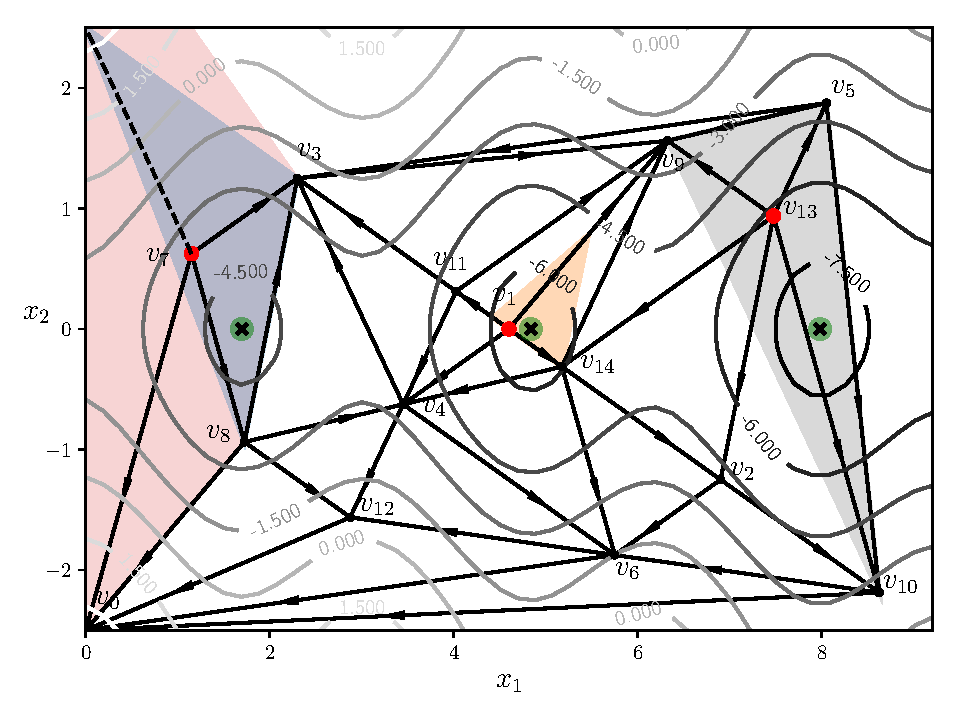
\includegraphics[scale=0.65]{./Fig9.pdf}}
{\caption{Visual demonstration of the proof by finding simplices with Sperner labellings. The three circled crosses are the (approximate) minimima of the objective function within the given bounds. The three possible Sperner simplices are contained within the star domains of each minimiser $\textrm{st}\left(v_{1}\right)$, $\textrm{st}\left(v_{7}\right)$ and $\textrm{st}\left(v_{13}\right)$. $v_{7}$ is an example of simplices without complete Sperner labelings, the red shaded area around $\overline{v_7}$ is the bounded domain wherein at least one local minimum exist
} \label{fig:Sperner}} 
\end{figure}

Note that if the edge $\overline{v_{13} v_{14}}$ was chosen instead of $\overline{v_{13}  v_{10}}$ then the local minimum of the function would be outside the domain of the simplex with the Sperner labelling. This is an important observation because it demonstrates that \autoref{theor:stat} cannot be used to further refine the location of the local minimum from the domain $\textrm{st}\left(v_{13}\right)$ using mechanisms of the proof, it only states that at least one local minimum exists within $\textrm{st}\left(v_{13}\right)$.

The boundaries of $\textrm{st}\left(v_{13}\right)$ can be found using the $3-$chain $C_{13}(\mathcal{H}^3)$ of simplices in $\textrm{st}\left( v_{13} \right)$, recall that the directions of simplices higher than dimension 2 are undefined and so the directions can be arbitrarily chosen $$C_{13}(\mathcal{H}^3) = \overline{v_{13} v_{10} v_{5}} + \overline{v_{13} v_{5} v_{9}} + \overline{v_{13} v_{9} v_{14}} + \overline{v_{13} v_{14} v_{2}} + \overline{v_{13} v_{2} v_{10}}$$

$C_{13}(\mathcal{H}^3)$ clearly forms a cycle, applying the boundary operator we find the faces defining the bounds of the domain of $\textrm{st}\left( v_i \right)$ which in this case is the chain of edges with defined direction  $$\partial(C_{13}(\mathcal{H}^{3})) = - \overline{ v_{10} v_{5}} + \overline{v_{5} v_{9}} - \overline{v_{9} v_{14}} + \overline{v_{14} v_{2}} + \overline{v_{2} v_{10}} $$ thus $\partial\left(\partial(C(\mathcal{H}^{3}))\right) = \emptyset$. 

$v_{7} = (1.15, 0.625)$ is an example of a minimiser that does not have all three required directions for a Sperner labelling, the light red shaded area represents the area wherein a local minimum can exist. For example on the lines $x_1 = 0$ for $x_2 \in [0.625, 2.5]$ or $x_2 = 2.5$ for $x_1 \in [0, 1.15]$ there will either exist a point $\bold{p}$ where the gradient $\nabla f (\bold{p})$ points in any direction pointing towards $[\frac{3}{2} \pi, 0)$ in which case and edge $\overline{v_{13} \bold{p}}$ exists that points in the $[\frac{\pi}{2}, \pi)$ direction and we have a simplex with a Sperner labelling. For example the dotted line on \autoref{fig:Sperner} with the Sperner simplex represented by blue shaded around $v_7$. If such a point does not exists then all points on those lines points in the $[0, \frac{3}{2} \pi)$ direction and so one or more local minimum lies somewhere on the boundary which is within the defined area.

%Note that while the extreme vertices where not sampled by the Sobol sequence (except for $v_0$), the bounds can be arbitrarily connected to the complex as was done with dotted edge connecting to $v_7$ to cover the entire search space.

There have been several developments in the extension of this lemma which could prove useful in applications extending the SHGO algorithm. One of the most interesting is by \citet{DeLoera2002} where they proved the Atanassov conjecture \cite{atanassov1996sperner} that for any polytope with $N$ vertices there are $N - n$ simplices that receive a complete set of Sperner labels. \citet{Meunier2006} further extended this theorem and more recently \citet{Musin2015} extended the theorems to a large class of manifolds with or without boundary. These theorems could prove useful for extending the algorithm to make use of this information. 
%More explicitly the Atanassov conjecture can be used to find how many stationary points exist in a domain larger than the simplices extracted from SHGO.
More explicitly, SHGO currently uses knowledge of the objective function evaluations, but only in a Boolean sense (in the form of directed edges). The theorems by Meunier and Musin allow us to extend Sperner's lemma to a simplicial complex built in a $(n+1)$-dimensional non-euclidean space. This would allow the application of ideas from discrete differential geometry. For example the Gauss-Bonnet theorem holds for discrete simplicial surfaces \cite{Crane2013DGP}. The Gauss-Bonnet theorem provides a relation between the total Gaussian curvature and the Euler characteristic of a surface. By simple summation of the angle defect around every vertex we can determine the Euler characteristic of a continuous surface. As will be demonstrated in Section 5.4 the simplicial complex used by SHGO is homeomorphic to complexes built on other topological hypersurfaces. Therefore when using explicit coordinates of the expected homomorphism the summation can be used to compare the error with the Euler characteristic which provides a metric for how accurately the objective function surface has been sampled. In global optimisation theory a simplicial complex built in this space can be used for approximating local and global Lipschitz constants for an objective function while still retaining the ability to detect locally convex sub-domains in the search space. %When the objective function is Lipschitz smooth ! discrete differential geometry \cite{Crane2013DGP}.


%%% Invariance
\section{Invariance of the directed complex within a bounded rectangle} \label{sec:invariance}

We now have a guarantee of finding stationary points in sub-domains near stationary points. However, we would also like to ensure that SHGO does not generate more than one minimiser starting point per convex sub-domain. This can only be guaranteed when an objective function surface is "adequately sampled". For black box functions there is no way to know if the number and distribution of sampling points is adequate without more information (for example if the number of local minima are known in the problem). However, it is an important property of the algorithm that $|\mathcal{M}|$ will stop increasing with higher sampling after this point. First we define an adequately sampled surface.

\begin{definition}
Consider a simplicial complex $\mathcal{H}$ built on an objective function $f$ with a compact feasible set $\Omega$ using Definitions \ref{def:h1} through \ref{def:h4}. The surface is said to be \bf{adequately sampled} \normalfont if there is one and only one true stationary point within every domain defined by \autoref{theor:stat}.
\end{definition}

The remainder of this section is devoted to proving the following theorem which holds in the case where $\Omega = [\mathbf{l}, \mathbf{u}]^n$.

\begin{theorem} \label{theorem:invariance_M} (Invariance of an adequately sampled simplicial complex $\mathcal{H}$) For a given continuous objective function $f$ that is adequately sampled by a sampling set of size $N$. If the cardinality of the minimiser pool extracted from the directed simplex $\mathcal{H}$ is $|\mathcal{M}|$. Then any further increase of the sampling set $N$ will not increase $|\mathcal{M}|$.
\end{theorem}

\begin{proof}
The proof relies on a homomorphism between the simplicial complex $\mathcal{H}$ constructed in the bounded hyperrectangle $\Omega$ and the homology (mod 2) groups of a constructed surface $\mathcal{S}$ on which we can invoke the invariance theorem.

Define the $n$-torus $\mathcal{S}_0$ from the compact, bounded hyperrectangle $\Omega$ by identification of the opposite faces and all extreme vertices. Now for every strict local minimum point $\bold{p} \in \Omega$ puncture a hypersphere and after appropriate identification the resulting $n$-dimensional manifold $\mathcal{S}_g$ is a connected g sum of g tori $S := S_0\,\#\,S_1\,\#\,\cdots\,\#\,S_{g - 1} \qquad  (g\text{ times})$

Any triangulation $\mathcal{K}$ of the topological space $\mathcal{S}$ is homeomorphic to $\mathcal{S}$, $\bold{H}_k(\mathcal{K}) \cong \bold{H}_k(\mathcal{S}) ~\forall k \subset \mathbb{Z}$. Note that this homomorphism is for a mod 2 homology between a triangulation $\mathcal{K}$ and the surface $\mathcal{S}$ and is thus undirected. A triangulation corresponding to all vertices and faces of $\mathcal{K}$ can be directed according to \autoref{def:h1}, \autoref{def:h2} and \autoref{def:h3} providing the directed simplicial complex $\mathcal{H}$. By construction we have, for an adequately sampled simplicial complex $\mathcal{H}$, an equality which exists between the cardinality of $\mathcal{M}$ and the Betti numbers of $\mathcal{S}$ as $|\mathcal{M}| = h_1 = rank (\bold{H}_1(\mathcal{S})) = rank (\bold{H}_1(\mathcal{K}))$. Here we invoke the invariance theorem

\begin{theorem} (Invariance theorem\cite{Henle1979}) %(Henle p. 154) 
The homology groups associated with a triangulation $\mathcal{K}$ of the a compact, connected surface $\mathcal{S}$ are independent of $\mathcal{K}$. In other words, the groups $\bold{H}_0 (\mathcal{K})$, $\bold{H}_1 (\mathcal{K})$ and $\bold{H}_2 (\mathcal{K})$ do not depend on the simplices, incidence coefficients, or anything else arising from the choice of the particular triangulation $\mathcal{K}$; they depend only on the surface $\mathcal{S}$ itself.
\end{theorem}
The invariance theorem can be extended to higher dimensional triangulable spaces using singular homology through the Eilenberg-Steenrod Axioms \cite{eilenberg47foundations, Henle1979}. As a direct consequence any triangulation of $\mathcal{S}$ will produce the same homology groups for $\mathcal{K}$.

Adding any new sampling point within the corresponding subdomains of $\textrm{st}\left( v_i \right)$ $ \forall i (v_i \in \mathcal{M} \subseteq \mathcal{H}^0 ) $ as defined in \autoref{theor:stat} will by definitions \ref{def:h1} through \ref{def:h4} need to be connected directly to $v_i$ by a new edge or the triangulation is no longer a simplicial complex and thus not increase $|\mathcal{M}|$ since only one vertex will be the new minimiser.

After adding any sampling point outside a domain $\textrm{st}\left( v_i \right)$ then, through the established homomorphism, any construction of $\mathcal{H}$ will produce the same homology groups since $rank (\bold{H}_1(\mathcal{K}))$ remains unchanged and it is thus not possible for a new vertex to be wrongly identified as a minimiser in the triangulation $\mathcal{H}$.

This concludes the proof that any increase in $N$ will not further increase $|\mathcal{M}|$.
\end{proof}


It is important to note that \autoref{theorem:invariance_M} is only applicable to complexes with adequate sampling as defined, that is to say it is entirely possible that, in complexes with less that adequate sampling, two starting minimiser elements of $\mathcal{M}$ will converge to the same local minimum. This flaw is inherent in the fact that there is insufficient information to completely identify the minima of a surface (and could be overcome if some extra information about $f$ is known).

%The set of sampling vertices $\mathcal{H}_0$ is directly related to the complex $\mathcal{F}$ by the boundary operator in the obvious way $\Omega \overset{\partial}{\leftarrow } \mathcal{F}_1 \overset{\partial}{\leftarrow } \mathcal{F}_2 \dots \overset{\partial}{\leftarrow } \mathcal{F}_n$. By puncturing the minimisers (formally defined as the toroidal points of the directed graph $\mathcal{F}_1$) in $\mathcal{F}$ a homomorphism to the homology (mod 2) groups $\mathcal{F}_k \cong\mathcal{H}_k ~\forall k \subseteq \mathbb{Z}$ can be formed which can be used as an approximate characterisation of the objective function $f$. An iterative procedure is used to apprimate the characterisation to a preset tolerance.

\autoref{theor:stat} and \autoref{theorem:invariance_M} also lead to the following corollary about an optimisation problem:

\begin{corollary} \label{corollary:smooth}
Consider any objective function $f : \Omega \subseteq \mathbb{R}^n \rightarrow \mathbb{R}$. Consider also a local minimisation routine that is guaranteed to converge to a local minimum in the same locally convex domain as the starting point inputted to the algorithm. Alternatively the local minimisation routine is guaranteed to converge to a point within a set of bounds (provided by the boundary of the $k-$chain around $\textrm{st}\left( v_i \right)$,  $\partial \left( C(\mathcal{H}^k) \right), k = n + 1$). If such a local minimisation routine  uses an element $v_i \in \mathcal{M}$ as a starting point and the routine leads to a minimum outside or on $\textrm{st}\left(v_{i}\right)$ and in addition the minimum is not contained in the set $\mathcal{H}^0$. Then it can be concluded that either search space is not adequately sampled or $f$ is not a Lipschitz smooth function.
\end{corollary}
Therefore according to \autoref{corollary:smooth} if the number of local minima are known, as in for example phase equilibria problems, then we can extract valuable information about the objective function. In particular it can be determined whether or not the objective function is Lipschitz smooth. Alternatively if the function is known to be Lipschitz smooth then \autoref{corollary:smooth} can be used to prove the sampling is insufficient when the condition is not met. When this happens it is also now known that there are more local minima to be found, one or more of which might possibly be the global minimum. \autoref{corollary:smooth} does not, however, provide any guarantee that the sampling is sufficient when the conditions are met.

\section{Sampling generation}
%\subsection{Sobol sampling}
Using the Sobol sequence sampling point generation proceeds in a similar way as that described in \Cref{sec:tgo1}. However, rather than only generating an arbitrary number of predefined sampling points we will also consider heuristic methods starting with the minimum amount of sampling points required to triangulate an $n$-dimensional space. For example start with the minimum amount of sampling points to construct an $n$-dimensional simplex and continue sampling while continuously calculating the $\bold{H}_1 (\mathcal{H})$ homology groups of the complex. Using the definitions described in this section the sampling is continued until the growth rate of the approximated homology groups slows appreciably. %This latter method is described in !!.

%\subsection{Minimum triangulation sampling}
%In this publication we also consider another uniform sampling which is generated from an algorithm using the symmetry group $S_n$ of the set $\{1, 2, 3, \dots, $n$\}$. This method is described in more detail Section \ref{sec:triangle}, but first we describe how the triangulation is used to construct the directed simplicial complex $\mathcal{H}$.
%\subsection{Triangulation}

%\section{Simplical constructions}



%\section{Triangulation methods} \label{sec:triangle}
%\subsection{Delaunay triangulation of Sobol points}
%!!TODO: Describe Delaunay triangulation. Provide references to Qhull library etc.
In this publication the Sobol sequenced sampling points are triangulated using Delaunay triangulation as implemented in the SciPy library \cite{scipy}. A major disadvantage to this triangulation scheme is that it does not scale well to higher dimensions since it relies on solving convex hull using the quickhull method developed by \citet{Barber1996}. %!!TODO add references to quickhull method scaling if there are any
There are several possibilities for mitigating this problem. Since the Sobol sequence is deterministic the triangulations can be calculated and stored in a database. For SHGO another possibility whereby the convex hull does not need to be solved by using symmetry generated triangulation was developed. Building on the initial $n$-cube triangulation developed by \citeauthor{paulavivcius2014simplicial} \citep{paulavivcius2014simplicial, Zilinskas2016} and using the symmetry groups $S_n,$ $n = \{1, 2, 3, \dots, $n$\}$ to generate an initial triangulation. Subsequent uniform sampling that ensures a symmetrical triangulation is generated in the next generation of simplices. This is done by an ordering of edges and using the cycle $(123 \dots n-1)$ to ensure that we always split every simplex by a hyperplane that goes through a new (child) vertex on the longest edge of simplex and every other vertex in the parent simplex that does not have incidence on the edge. Figure \ref{fig:triangles} demonstrates the symmetry of this sampling in $n=2$ where the longest edge in the initial triangulation was sampled. Here an iteration is defined as any generation of sub-triangulations that provides a triangulation symmetrical to the initial triangulation. An implementation of this sampling sequence is available at \citet{SHGOpy}.

\begin{figure}
\centerline{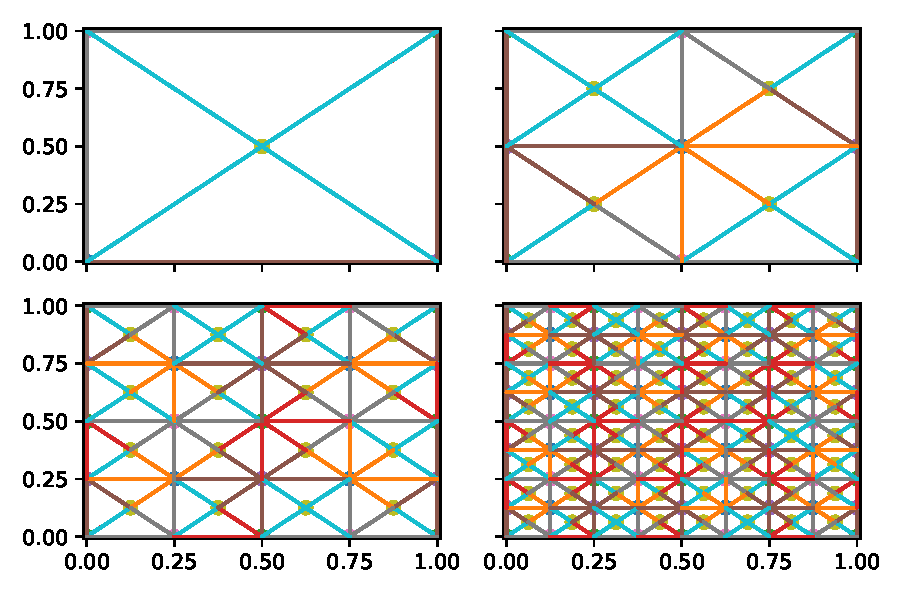
\includegraphics[scale=1.0]{./Fig10.pdf}}
{\caption{Triangulation of a unit hypercube shown in 2 dimensions for 4 iterations  \label{fig:triangles} }}
\end{figure}

In this publication we will use both the Sobol and the hypercube triangulation sampling sequences. Sobol provides a more direct comparison to the TGO algorithm while the second sequence is more similar to the DISIMPL-v algorithm. We will refer to the different uses of sampling sequences as SHGO-Sobol and SHGO-Simpl in the experimental results in \Cref{sec:results}.

\section{Invariance and convergence of non-continuous, non-linear optimisation problems with bounded variables}
In this section we again consider \Cref{eq:gen_op}, but now consider the case where $\mathbf{g}$ is non-linear. In addition we allow $f$ to be non-continuous (in having removable or jump discontinuities) and non-linear. It is still assumed that the variables $\mathbf{x}$ are bounded. Furthermore we assume that there is a feasible solution so that $\Omega \neq \emptyset$ and that there exists at least point in range of $f$ mapped within the domain $\Omega$. We will prove that if the simplicial sampling sequence \citep{SHGOpy} is used, then SHGO will retain the Invariance property of \Cref{theorem:invariance_M}. Secondly convergence of the SHGO algorithm is proved when the number of sampling points tends to infinity.

Before proving these properties we will need to define a new construction to deal with discontinuities in $f$. From \Cref{def:h0} and \Cref{def:h0.5} it is clear that $f$ will only map a subset of feasible domain $\Omega$, therefore only points within the this domain need to be considered. A new construction replacing \Cref{def:h0.5} that considers discontinuities (such as singularities) in the hypersurface of $f$ is now defined:

\begin{definition} \label{def:hnew}
For an objective function $f$, $\mathcal{F}$ is the set of scalar outputs mapped by the objective function $f:\mathcal{P} \rightarrow \mathcal{F}$ for a given sampling set $\mathcal{P} \subseteq \Omega \subseteq \mathbb{R}^n$. If a mapping of a vertex $v_i$ does not exist, then we define the mapping as $f: v_i \rightarrow \infty$.  Any such point is excluded from the set $\mathcal{M}$.
\end{definition}

Note from \Cref{def:h3} that any vertex $v$, $f(v) = \infty$ that is connected to another vertex in $\Omega$ that maps to a finite value will never be a minimiser.

\begin{theorem} \label{theorem:invariance_n} (Invariance of an adequately sampled simplicial complex $\mathcal{H}$ in a non-convex, non-compact space $\Omega$) For a given non-continuous, non-linear objective function $f$ that is adequately sampled by a sampling set of size $N$. If the cardinality of the minimiser pool extracted from the directed simplex $\mathcal{H}$ is $|\mathcal{M}|$. Then any further increase of the sampling set $N$ will not increase $|\mathcal{M}|$.
\end{theorem}

\begin{proof}
\Cref{theorem:invariance_M} holds for any compact hyperrectangular space $\mathbb{B}_0 = [x_l^1, x_u^1] \times [x_l^2, x_u^2] \times \dots \times [x_l^n, x_u^n]$. Consider a set of subspaces $\mathbb{B}_i \cong \mathbb{B}_0 $ with $\mathbb{B}_i \subseteq \Omega ~\forall i \in \mathbf{I}$. That is, $\mathbb{B}_i$ is any compact, rectangular subspace of $\Omega$ that is homeomorphic to $\mathbb{B}_0$ (which is also homeomorphic to a point) and can, therefore, be shrunk or expanded to arbitrary sizes while retaining compactness. Therefore any triangulation $\mathcal{K}_i$ of $\mathbb{B}_i$ retains the Invariance property from \Cref{theorem:invariance_M}. 

We allow all $\mathbb{B}_i$ to be connected or disconnected subspaces with respect to any other $\mathbb{B}_{j \in I}$ within $\Omega$. Now consider the (mod 2) homology groups $\bold{H}_1(\mathcal{K}_i)$ of $\mathcal{K}_i$. Since the homology groups are abelian groups the rank is additive over arbitrary direct sums:
$$
\operatorname{rank}\left(\bigoplus_{i\in I}\bold{H}_1(\mathcal{K}_i)\right) = \sum_{i \in I}\operatorname{rank}(\bold{H}_1(\mathcal{K}_i))
$$
Therefore the triangulations of both connected and disconnected subspaces $\mathbb{B}_i$ within a possibly non-compact space $\Omega$ will retain the same total rank. After adequate sampling, the rank of $\bold{H}_1(\mathcal{K}_i)$ will not increase by \Cref{theorem:invariance_M}. Any point that is not in $\Omega$ is not connected to any graph structure by \Cref{def:h0} and \Cref{def:h0.5} and therefore cannot increase the rank of any homology group $\bold{H}_1(\mathcal{K}_i)$. Finally any vertex $v_i \in \Omega$ for which $f(v_i)$ does not exist will by \Cref{def:hnew} be mapped to infinity by \Cref{def:hnew}. By \Cref{def:h4}, $v_i$ can not be a minimiser and therefore cannot increase the rank of any homology group $\bold{H}_1(\mathcal{K}_i)$. For the reader's benefit \Cref{fig:nonlinear3} demonstrates this property geometrically.

We have shown that the total rank of the homology groups triangulated on all connected and disconnected subspaces $\mathbb{B}_i \in \Omega$ will not increase after adequate sampling. It remains to be proven that these subspaces exist within $\Omega$. We adapt the convergence proof used by \citet{Paul2014a} for subdivided simplicial complexes. 
\begin{proposition}
For any point $\mathbf{x} \in \Omega$ and any $\epsilon > 0$ there exists an iteration $k(\epsilon) \ge 1$ and a point $\mathbf{x}_i^k \in \mathcal{H}^n \in \Omega$ such that $\norm{\mathbf{x}_i^k - \mathbf{x}} < \epsilon$.
\end{proposition}
Sampling points $\mathbf{x}_i$ are vertices $\mathcal{H}^0$ belonging to the set of $n$-dimensional simplices $\mathcal{H}^n$. Let $\delta^k_{max}$ be the largest diameter of the largest simplex. Since the subdivision is symmetrical all simplices have the same diameter $\delta^k_{max}$ after every iteration of the complex. At every iteration the diameter will be divided through the longest edge, thus reducing the simplices' volumes. After a sufficiently large number of iterations all simplices will have the diameter smaller than $\epsilon$. Therefore the vertices of the complex will converge to any and all points inside compact subspaces $\mathbb{B}_i$ within $\Omega$. Since we have assumed that $\Omega \neq \emptyset$ this proves the existence of subspaces $\mathbb{B}_i$. 

This concludes the proof of \Cref{theorem:invariance_n}
\end{proof}
From this proof the convergence to a global minimum within $\Omega$, if it exists, also trivially follows by noting that $\mathbb{B}_i$ is homeomorphic to a point and that \Cref{theor:stat} applies to any minimiser in $\mathbb{B}_i$. In practice \Cref{def:hnew} is implemented in \citet{SHGOpy} by using exception handling that can capture any mathematical errors in addition to converting any none float numbers outputted by an objective function to infinity objects.

\begin{figure} 
\centerline{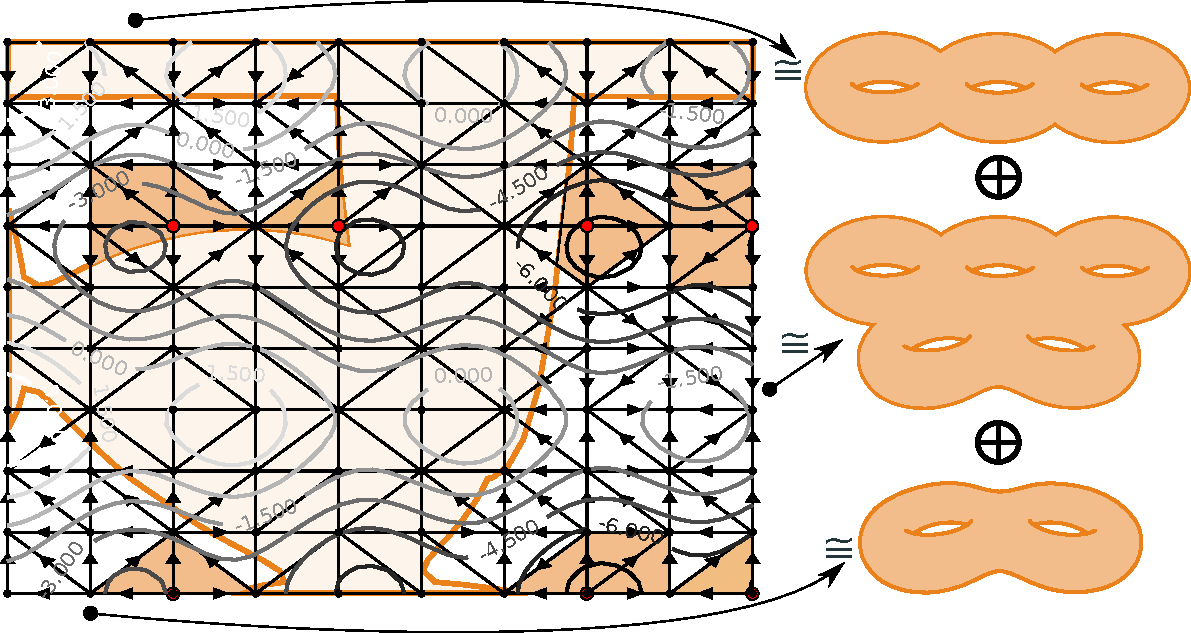
\includegraphics[scale=0.85]{./non_linear_3.pdf}}
{\caption{Visual demonstration on surfaces with non-linear constraints, the shaded region is unfeasible. The vertices of the points mapped to infinity have undirected edges, therefore they do not form simplicial complexes in the integral homology. The surfaces of each disconnected simplicial complex $\mathcal{K}_i$ can be constructed from the compact version of the invariance theorem. The rank of the abelian homology groups $\bold{H}_1(\mathcal{K}_i)$ is additive over arbitrary direct sums\label{fig:nonlinear3}}}
\end{figure}


\section{Theoretical comparison to the DISIMPL algorithm}
The DISIMPL algorithm developed by \citeauthor{Paul2014b} \citep{Paul2014b, paulavivcius2014simplicial, Paul2014a} is based on spatial partitioning of the search space. DISIMPL-v in particular should have a similar initial complex as SHGO-Simpl for box problems since this algorithm samples on the vertices of the simplicial complex (while DISIMPL-c samples at the geometric centre of the simplices which is more appropriate for higher dimensional problems). The graph structure of DISIMPL-v can thus be used to construct the directed complex $\mathcal{H}$ and the homological properties can be calculated and applied. An example of one such application is given in the following paragraph.

At every iteration of the DISIMPL algorithm potentially optimal simplices are selected for refinement by considerations the Lipschitz properties of the optimisation problem. In general a combination of promising simplices with good function evaluations (related to local exploration of the search space) and simplices with larger hypervolumes (related to global exploration of the search space). Gb-DISIMPL \citep{Paul2014a} is a very promising acceleration technique accomplished by switching between a "global phase" and a "usual phase". The global phase is focused on exploring simplices with larger hyper volumes and excludes smaller simplices which are potentially optimal in the usual phase. This technique prevents excessive evaluations near local minima as demonstrated in \citet{Paul2014a}. Local minima can put a "drag" on the progress of refining the minimum because the algorithm selects many neighbouring simplices that are slightly worse on the function values, but also slightly larger in volume. A meta-parameter is used in Gb-DISIMPL to select the simplices to be excluded in the global phase and was shown in \citet{Paul2014a} to be very efficient. However, using knowledge from the directed complex of $\mathcal{H}$, the domain containing these simplices near the local minima could also be identified more explicitly through a Sperner labelling if the function is known to be Lipschitz smooth.

%!!TODO: Also show the proof of the inherent lower limit of maintaining mod 2 information relating the vertices in higher dimensions (~ 10 lines) (NEXT PAPER)

%!!TODO: Mentiond the 3 triangulation schemes of the n-cube ($D_3$ etc.)

%!!TODO: Use subplots for these

%\begin{figure} \label{fig:3dg0}
%\centerline{\includegraphics[scale=0.65]{../6shgo/img/3dgen1.pdf}}
%{\caption{The initial triangulation of the 3-cube generated from the symmetry group $S_3$}}
%\end{figure}

%\begin{figure} \label{fig:3dg2}
%\centerline{\includegraphics[scale=0.65]{../6shgo/img/3dgen2.pdf}}
%{\caption{The second generation of the 3-cube generated from hyperplane cuts using the symmetry groups $S_3$ and $S_2$}}
%\end{figure}

%\begin{figure} \label{fig:3dg10}
%\centerline{\includegraphics[scale=0.65]{../6shgo/img/3dgen10.pdf}}
%{\caption{The tenth generation of the 3-cube generated from hyperplane cuts using the symmetry groups $S_3$ and $S_2$}}
%\end{figure}

%\begin{figure} \label{fig:2dg1}
%\centerline{\includegraphics[scale=0.65]{../6shgo/img/2dgen1.pdf}}
%{\caption{The initial triangulation of the 2-cube generated from the symmetry group $S_2$}}
%\end{figure}

%\begin{figure} \label{fig:2dg2}
%\centerline{\includegraphics[scale=0.65]{../6shgo/img/2dgen2.pdf}}
%{\caption{The second generation of the 2-cube generated from hyperplane cuts using the symmetry groups $S_2$ and $S_1$}}
%\end{figure}

%\begin{figure} \label{fig:3dg10}
%\centerline{\includegraphics[scale=0.65]{../6shgo/img/2dgen10.pdf}}
%{\caption{The tenth generation of the 2-cube generated from hyperplane cuts using the symmetry groups $S_2$ and $S_1$}}
%\end{figure}

%\section{Properties of complex and invariance theorem}
%\section{Homomorphisms to mod 2 homology groups}
%(For function characterisation)



\section{Algorithm implementation}
We consider two modes for the SHGO algorithm. In the first a finite number of sampling points $N$ are specified and sampling is continued until an $\Omega$ set of cardinality $N$ is produced and no further sampling occurs. This method is demonstrated by Algorithm \ref{alg:shgo1}. The main reason for this algorithm is to present a more direct comparison to TGO that can be used in numerical experiments.% we will use Algorithm \ref{alg:shgo1} in the numerical experiments.

For the purposes of global optimisation and local minima exploration Algorithm \ref{alg:shgo2} is more appropriate. By continuously calculating the $\bold{H}_1 (\mathcal{H})$ homology group several termination criteria can be used to end the sampling. For example if the amount of local minima is known the sampling can be terminated once $|\mathcal{M}|$ is large enough. Another example with many possible heuristics is tracking the historical difference in $|\mathcal{M}|$ over $|\mathcal{P}|$ and terminating sampling if $|\mathcal{M}|$ is unchanged after a certain increase in $|\mathcal{P}|$. In optimisation problems where the global minimum is known we can also use the stopping criteria such as the one defined by \citet{Paul2016}. 

\[ pe = 100\% \times \begin{cases} 
       \frac{\min\{\mathcal{F}\} - f^*}{|f^*|}, & f* \neq 0 \\
       \min\{\mathcal{F}\},  & f^* = 0
   \end{cases}
\]

Here $\min\{\mathcal{F}\}$ is the minimum function evaluation obtained including values obtained in the output of the local minimisation step as shown in the algorithm. Whatever termination criterion is used it requires an input $\bold{H}_1 (\mathcal{H})$ or $\min\{\mathcal{F}\}$ and should output a Boolean, we will refer to this function as $\mathbf{TERM}(\bold{H}_1 (\mathcal{H}), \min\{\mathcal{F}\})$ in Algorithm \ref{alg:shgo2}. In the practical implementation of the algorithm the user can also specify a finite number of iterations and/or sampling points. This functionality has been programmed into the $\mathbf{TERM}(\bold{H}_1 (\mathcal{H}), \min\{\mathcal{F}\})$ function.


Open source python implementations of both of these algorithms are available and were published under a MIT compatible license \citep{SHGOpy}.

\begin{algorithm} 
\caption{SHGO finite sampling algorithm}
\label{alg:shgo1}
\begin{algorithmic}[1]
\Procedure{Initialisation}{}
\State \bf{Input} \normalfont an objective function $f$, constraint functions $\mathbf{g}$ and variable bounds and $[\mathbf{l}, \mathbf{u}]^n$.
\State \bf{Input} \normalfont $N$ initial sampling points.
\State Define a sampling sequence that generates a set $\mathcal{X}$ of sampling points in the unit hypercube space $[\mathbf{0}, \mathbf{1}]^n$
\EndProcedure
\Procedure{Initial sampling}{}
\State $\mathcal{P} = \emptyset$
\While{$|\mathcal{P}|$ $<$ $N$}
\State Generate $N - |\mathcal{P}|$ sequential sampling points $\mathcal{X} \subset \mathbb{R}^n$
\State Stretch $\mathcal{X}$ over the lower and upper bounds $[\mathbf{l}, \mathbf{u}]^n$
\State  $\mathcal{P} = \{\mathcal{X}_i ~|~ \mathbf{g}(\mathcal{X}_i) \geq 0, \forall \mathcal{X}_i \in \mathcal{X}\} \cup\mathcal{P}$ 
\Comment (Find $\mathcal{P}$ in the feasible subset $\Omega$ by discarding any points mapped outside the linear constraints $g$ and adding to the current set of $\mathcal{P}$.)
\State Set $\mathcal{X} = \emptyset$
\EndWhile
\State Find $\mathcal{F}$ from the objective function $f: \mathcal{P} \rightarrow \mathcal{F}$
\EndProcedure
\Procedure{Construct directed complex $\mathcal{H}$}{}
\State Calculate $\mathcal{H}$ from $h: \mathcal{P}\rightarrow \mathcal{H}$
\EndProcedure
\Procedure{Construct $\mathcal{M}$}{}
\State Find $\mathcal{M}$ from \Cref{def:h4}.
\EndProcedure
\Procedure{Local minimisation}{}
\State Calculate the approximate local minima of $f$ using a local minimisation routine with the elements of $\mathcal{M}$ as starting points.
\Comment These local minimisations can be performed in parallel.
\EndProcedure
\Procedure{Process return objects}{}
\State Order the final outputs of the minima of $f$ found in the local minimisation step to find the approximate global minimum.
\EndProcedure \\
\Return the approximate global minimum and a list of all the minima found in the local minimisation step.
\end{algorithmic}
\end{algorithm} 





\begin{algorithm} 
\caption{SHGO homology group growth algorithm}
\label{alg:shgo2}
\begin{algorithmic}[1]
\Procedure{Initialisation}{}
\State \bf{Input} \normalfont an objective function $f$, constraint functions $\mathbf{g}$ and variable bounds and $[\mathbf{l}, \mathbf{u}]^n$.
\State \bf{Input} \normalfont $N$ initial sampling points.
\State Define a sampling sequence that generates a set $\mathcal{X}$ of sampling points in the unit hypercube space $[\mathbf{0}, \mathbf{1}]^n$
\State Define the empty set $\mathcal{M}^E = \emptyset$ of vertices evaluated by a local minimisation.
\EndProcedure
\While{$\mathbf{TERM}(\bold{H}_1 (\mathcal{H}), \min\{\mathcal{F}\})$ is False}
\Procedure{Sampling}{}
\State $\mathcal{P} = \emptyset$
\While{$|\mathcal{P}|$ $<$ $N$}
\State Generate $N - |\mathcal{P}|$ sequential sampling points $\mathcal{X} \subset \mathbb{R}^n$
\State Stretch $\mathcal{X}$ over the lower and upper bounds $[\mathbf{l}, \mathbf{u}]^n$
\State  $\mathcal{P} = \{\mathcal{X}_i ~|~ \mathbf{g}(\mathcal{X}_i)  \geq 0, \forall \mathcal{X}_i \in \mathcal{X}\} \cup\mathcal{P}$ 
\Comment (Find $\mathcal{P}$ in the feasible subset $\Omega$ by discarding any points mapped outside the linear constraints $g$ and adding to the current set of $\mathcal{P}$.)
\State Set $\mathcal{X} = \emptyset$
\EndWhile
\State Find $\mathcal{F}$ from the objective function $f: \mathcal{P} \rightarrow \mathcal{F}$ for any new points in $\mathcal{P}$
\EndProcedure
\Procedure{Construct/append  directed complex $\mathcal{H}$}{}
\State Calculate $\mathcal{H}$ from $h: \mathcal{P}\rightarrow \mathcal{H}$  
\Comment (If $\mathcal{H}$ was already constructed new points in $\mathcal{P}$ are incorporated into the triangulation.)
\State Calculate $\bold{H}_1 (\mathcal{H})$
\EndProcedure
\Procedure{Construct $\mathcal{M}$}{}
\State Find $\mathcal{M}$ from \Cref{def:h4}.
\EndProcedure
\Procedure{Local minimisation}{}
\State Calculate the approximate local minima of $f$ using a local minimisation routine with the elements of $\mathcal{M} \setminus \mathcal{M}^E$ as starting points. 
\Comment Process the most promising points first.
\State $\mathcal{M}^E = \mathcal{M}^E \cap \mathcal{M}$  \Comment This excludes the evaluation any element $ v_i \in \mathcal{M}$ that is known to be the only point that in the domain $\partial \textrm{st}(v_j)$ where $v_j$ is known to any point already used as a starting point in Step 27. If any new $ v_i \in \mathcal{M}$ not in $\mathcal{M}^E $ is known to be the only point $\partial \textrm{st}(v_j)$ it can also be excluded.
\State Add the function outputs of the local minimisation routine to $\mathcal{F}$
\EndProcedure
\State Find new value of $\mathbf{TERM}(\bold{H}_1) (\mathcal{H}, \min\{\mathcal{F}\})$
\EndWhile
\Procedure{Process return objects}{}
\State Order the final outputs of the minima of $f$ found in the local minimisation step to find the approximate global minimum.
\EndProcedure \\
\Return the approximate global minimum and a list of all the minima found in the local minimisation step.
\end{algorithmic}
\end{algorithm} 



%\section{Results}
\chapter{Experimental Results} \label{sec:results}
\section{Comparison to algorithms that can solve problems with linear constraints}

In this section we provide experimental comparisons on 22 linearly constrained problems comparing the SHGO, TGO, Lc-DISIMPL \citep{Paul2016}, PSwarm \citep{Vaz2008} and DIRECT-L1 \citep{finkel2003direct} algorithms. Note that the data for the Lc-DISIMPL, PSwarm and DIRECT-L1 algorithms was taken from \citet{Paul2016}. The same error of $pe = 0.01\%$ used by \citet{Paul2016} was also used in this publication. To provide a fair comparison of TGO to SHGO and the other solvers the TGO algorithm was modified to stop sampling when it produced a minimiser that lead to the global minimum of the problem. Table \ref{tab:lc_results} shows the results. Here f.e.\ is the total number of objective function evaluations required to solve the function and p.f.e. is the total number of penalty function evaluations. \citet{Paul2016} used DIRECT-L1 with the 3 different penalty parameters (p.p.) shown in the table. The PSwarm solver was run 10 times for each test problem. 

The SHGO-Simpl, SHGO-Sobol and TGO (using Henderson's formula for $k_c$) algorithms were able to solve all 22 problems. The lowest average number of function evaluations was achieved by SHGO-Simpl followed by SHGO-Sobol and TGO. It can be observed that Lc-DISIMPL-v achieved a better performance than any other algorithm for the horst-1 to horst-6, hs024, hs035, s232, s250 and bunnag2 problems. As noted in \citet{Paul2016} the initial triangulation of Lc-DISIMPL-v evaluates the function values at the vertices of the simplices and therefore for some of the tested problems the solutions were found after initial triangulation on one of the vertices of the feasible region. It is also possible to initiate SHGO with such an initial triangulation by definition the first few vertices in $\mathcal{X}$ as the intercepts of the linear constraints in a similar way to \citet{Paul2016} and then continuing to add sampling points as normal.

Table \ref{tb:lc} provides additional information for SHGO and TGO including the total number of function evaluations required by the algorithm to solve the problem (f.e.), the number of minimisers generated as starting points by the algorithm (nlmin), the number of unique local minima mapped by the algorithm (nulmin) and the total processing time (runtime) in seconds.

It can be seen that neither of the SHGO algorithms produced more starting points leading to the same local minima as predicted by the theory for adequately sampled function surfaces. On the contrary TGO produced more than one starting point in the same locally convex domain on some test problems which lead to extra function evaluations, producing a poorer overall performance. While SHGO-Simpl had the lowest number of average function evaluations, a higher processing run time is observed compared to the other 2 algorithms. This can be explained by the fact the triangulation code for the sampling has, not yet been optimised, which consumed most of the run time. SHGO-Sobol and TGO use the same sampling generation code and it is observed that SHGO-Sobol has a lower processing run time as expected.


The source code used to produce these results including the scripts that run the test benchmarking suite is publically available at \citet{SHGOpy}. The specifications of the system used to run the test problems can be found in Appendix~\ref{sec:nres}.



\setlength{\tabcolsep}{5.5pt}
\begin{landscape}
% \hspace*{-3cm} 
\begin{table}[htbp]
\caption{Function evaluation comparisons for test problems with linear constraints.}%The results for the Lc-DSIMPL, PSwarm and DIRECT-L1 algorithms were taken from \citet{Paul2016}}
%{\tablinesep=2ex\tabcolsep=10pt
\begin{tabular}{lrrrrrrrrrrrrrr}
\toprule
 & \multicolumn{1}{l}{shgo-}  & \multicolumn{1}{l}{} & \multicolumn{1}{l}{tgo}  & \multicolumn{2}{l}{Lc-DSIMPL-$^c$}   & \multicolumn{1}{l}{PSwarm$^c$} & \multicolumn{1}{l}{} & \multicolumn{1}{l}{} & \multicolumn{1}{l}{}  & \multicolumn{1}{l}{} & \multicolumn{1}{l}{} & \multicolumn{2}{l}{DIRECT-L1$^c$}  &  \\  \cmidrule(lr){7-12}
 & \multicolumn{1}{l}{-simpl}  & \multicolumn{1}{l}{-sobol} & \multicolumn{1}{l}{}  & \multicolumn{1}{l}{-v} & \multicolumn{1}{l}{-c} & \multicolumn{1}{l}{Minimum} & \multicolumn{1}{l}{} & \multicolumn{1}{l}{Average} & \multicolumn{1}{l}{} & \multicolumn{1}{l}{Maximum} & \multicolumn{1}{l}{} & \multicolumn{1}{l}{p.p. = 10} & \multicolumn{1}{l}{p.p. = 10$^2$} & \multicolumn{1}{l}{p.p.=10$^6$} \\  \cmidrule(lr){2-3} \cmidrule(lr){4-4}  \cmidrule(lr){5-6} \cmidrule(lr){7-8} \cmidrule(lr){9-10} \cmidrule(lr){11-12}  \cmidrule(lr){13-15}
Problem & \multicolumn{1}{l}{f.e.} & \multicolumn{1}{l}{f.e.} & \multicolumn{1}{l}{f.e.} & \multicolumn{1}{l}{f.e.} & \multicolumn{1}{l}{f.e.} & \multicolumn{1}{l}{f.e.} & \multicolumn{1}{l}{p.f.e} & \multicolumn{1}{l}{f.e.} & \multicolumn{1}{l}{p.f.e.} & \multicolumn{1}{l}{f.e.} & \multicolumn{1}{l}{p.f.e} & \multicolumn{1}{l}{f.e} & \multicolumn{1}{l}{f.e.} & \multicolumn{1}{l}{f.e.} \\ 
\midrule
horst-1  & 97 & 24 & 34 & \textbf{7} & 249 & 167 & 182 & 1329$^{b(3)}$ & 1343$^{b(3)}$ & 4100$^{b(3)}$ & 4101$^{b(3)}$ & 287$^a$ & 3689 & $>$100000 \\[0.05cm]
horst-2  & 10 & 11 & 11 & \textbf{5} & 171 & 160 & 176 & 424 & 492 & 768 & 867 & 265$^a$ & 10829 & $>$100000 \\[0.05cm]
horst-3  & 6 & 7 &  6 & \textbf{5} & 249 & 42 & 43 & 44 & 45 & 46 & 47 & 5$^a$ & 591 & 617 \\[0.05cm]
horst-4  & 10 & 25 & 24 & \textbf{8} & 260 & 90 & 179 & 114 & 194 & 129 & 211 & 58293$^a$ & $>$100000 & $>$100000 \\[0.05cm]
horst-5  & 20 & 15 & 15 & \textbf{8} & 259 & 106 & 150 & 134 & 192 & 214 & 302 & 7$^a$ & $>$100000 & $>$100000 \\[0.05cm]
horst-6  & 22 & 59 & 77 & \textbf{10} & 284 & 90 & 172 & 110 & 192 & 133 & 227 & 11$^a$ & 739$^a$ & $>$100000 \\[0.05cm]
horst-7  & \textbf{10} & 15 & 13 & \textbf{10} & 220 & 188 & 201 & 380 & 403 & 919 & 957 & 7$^a$ & 71$^a$ & $>$100000 \\[0.05cm]
hs021  & 24 & \textbf{23} & \textbf{23} & 189 & 133 & 110 & 110 & 189 & 192 & 392 & 405 & 97 & 97 & 97 \\[0.05cm]
hs024  & 24 & 15 & 36 & \textbf{3} & 141 & 101 & 153 & 118 & 172 & 138 & 195 & 19$^a$ & 57$^a$ & $>$100000 \\[0.05cm]
hs035  & 37 & 41 & \textbf{35} & 630 & 721 & 266 & 311 & 316 & 369 & 327 & 373 & $>$100000 & $>$100000 & $>$100000 \\[0.05cm]
hs036  & 105 & 20 & 103 & \textbf{8} & 314 & 179 & 179 & 396 & 401 & 561 & 574 & 25$^a$ & 49$^a$ & $>$100000 \\[0.05cm]
hs037  & 72 & \textbf{63} & 258 & 186 & 9129 & 127 & 131 & 160 & 167 & 201 & 574 & 7$^a$ & 7$^a$ & $>$100000 \\[0.05cm]
hs038  & \textbf{225} & 1029 & 389 & 3379 & $>$100000 & 53662 & 54445 & 58576 & 59821 & 65677 & 67660 & 7401 & 5885 & 6511 \\[0.05cm]
hs044  & 199 & 35 & 51 & \textbf{20} & 440 & 148$^{b(9)}$ & 218$^{b(9)}$ & 186$^{b(9)}$ & 281$^{b(9)}$ & 201$^{b(9)}$ & 299$^{b(9)}$ & 90283 & $>$100000 & $>$100000 \\[0.05cm]
hs076  & 56 & \textbf{37} & 44 & 548 & 4794 & 132 & 198 & 203 & 286 & 275 & 341 & 19135 & $>$100000 & $>$100000 \\[0.05cm]
s224  & 166 & 165 & 165 & \textbf{49} & 463 & 105 & 107 & 121 & 122 & 157 & 158 & 7$^a$ & 431 & 457 \\[0.05cm]
s231  & \textbf{99} & \textbf{99} & 383 & 2137 & 655 & 542 & 1011 & 2366 & 3020 & 4116 & 4800 & 1261 & 1209 & 43341 \\[0.05cm]
s232 & 24 & 15 & 22 & \textbf{3} & 141 & 105 & 144 & 119 & 171 & 162 & 236 & 19$^a$ & 57$^a$ & $>$100000 \\[0.05cm]
s250 & 105 & 20  & 103 & \textbf{8} & 314 & 296 & 296 & 367 & 375 & 495 & 498 & 25$^a$ & 49$^a$ & $>$100000 \\[0.05cm]
s251 & 72 & \textbf{63} & 258 & 186 & 9127 & 83 & 84 & 129 & 137 & 175 & 180 & 7$^a$ & 7$^a$ & $>$100000 \\[0.05cm]
bunnag1  & \textbf{34} & 47 & 39 & 630 & 721 & 132 & 142 & 214 & 228 & 411 & 438 & 1529 & 1495 & 1463 \\[0.05cm]
bunnag2  & 46 & 36 & 35 & \textbf{16} & 500 & 150 & 153 & 252 & 259 & 410 & 426 & $>$100000 & $>$100000 & $>$100000 \\[0.05cm]
\cmidrule(lr){2-15}
Average  & \textbf{66} & 88 & 100 & 366 & $>$5877 & 2590 & 2672 & 3011 & 3130 & 3637 & 3812 & $>$17213 & $>$28421 & $>$75113 \\[0.05cm]
\bottomrule
\end{tabular}
\begin{tabular}{l}
$a$ result is outside the feasible region \\
$b(t)$ $t$ out of 10 times the global solution was not reached \\
$c$ results produced by \citeauthor{Paul2016} (\citeyear{Paul2016})
\end{tabular}
%}
 \label{tab:lc_results}
\end{table}
\thispagestyle{plain}
\end{landscape}


\begin{table}[htbp]
\caption{Total and average performance over all 22 test problems.}
\begin{tabular}{llrrrr}
\toprule
    &                &  f.e. &  nlmin &  nulmin  &   runtime (s) \\
problem & name        &       &        &                  &           \\
\midrule
All & shgo-simpl     &  1463 &     26 &      26  &       0.27294 \\
    & shgo-sobol       &  1864 &     23 &      23 &       0.11225 \\
    & tgo       &  2123 &     29 &      25  &       0.093607 \\
Average & shgo-simplicial      &    65 &      1 &       1  &  0.012852 \\
    & shgo-sobol       &    88 &      1 &       1  &  0.004144 \\
    & tgo      &    100 &      1 &       1  &  0.004542 \\
\bottomrule
\end{tabular}
\label{tb:lc}
\end{table}

\section{Function evaluations and comparison to other open source global optimisation algorithms}
In this section we present numerical experiments comparing the SHGO and TGO algorithms with the SciPy implementations \citep{scipy} of basinhopping (BH) \citep{li1987monte, wales2003energy, wales1997global, wales1999global} and differential evolution (DE) \citep{Storn1997}. These algorithms were chosen both because the open source versions are readily available in the SciPy project and because BH is commonly used in energy surface optimisations \citep{Wales2015} from which the motivation for developing SHGO grew. DE has also been applied in optimising Gibbs energy surfaces for phase equilibria calculations \citep{Zhang2011}. The optimisation problems in Appendix~\ref{sec:nres} were selected from the SciPy global optimisation benchmarking test suite \citep{Adorio2005, Gavana2016, Jamil2013, Mishra2007, Mishra2006, NIST2016}. The test suite contains multi-modal problems with box constraints, they are described in detail in \citet{Gavana2016}. We again used the stopping criteria $pe = 0.01\%$ for SHGO and TGO. For the stochastic algorithms (BH and DE) the starting points provided by the test suite were used. For every test the algorithm was terminated if the global minimum was not found after 10 minutes of processing time and the test was flagged as a fail. For comparisons we used normalised performance profiles \citep{Dolan2002} using function evaluations and processing time as performance criteria. In total 180 test problems were used.

From \Cref{fig:pprofile} it can be observed that for this problem set SHGO-Sobol was the best performing algorithm, followed closely by TGO and SHGO-Simpl. \Cref{fig:pprofilezoom} provides a clearer comparison between these three algorithms. While the performance of all 3 algorithms are comparable, SHGO-Sobol tends to outperform TGO, solving more problems for a given number of function evaluations. This is expected since, for the same sampling point sequence, TGO produced more than one starting point in the same locally convex domain on some test problems which leads to extra function evaluations. In total TGO produced 403 minima of which only 393 minima were unique while all of the 225 minima produced by SHGO-Sobol were unique. SHGO-Simpl produced 238 of which all 238 were unique. It is apparent that SHGO-Simpl performed worse compared to the other sampling methods despite a better performance on the test problem set with linear constraints. There are two reasons for this result. First of all, the uniformity properties of the Sobol sequence hold only for hypercubes. Therefore, it is lost for geometries defined by the search spaces inside linear constraints. Secondly the current code for the triangulation of the simplex cannot add only one sampling point per iteration, but must split all the simplices until the symmetry of the entire complex is restored. This leads to a much higher number of function evaluations during the sampling step of the algorithm.

\Cref{tab:results} in Appendix~\ref{sec:nres} shows the raw numerical results. Note that, unlike the data in performance profiles, failed test runs did not get set to the worst case performance criteria by any solver (in order to preserve the raw data). Therefore the total and average function evaluations and processing times are misleading. The Table is mostly useful for comparisons on a particular test problem as well as comparing the total number of minima and unique minima found.



%From the results it should first be noted that not all of the 1035 starting minimisers produced by SHGO algorithm lead to unique local minima (of which  944 is found across all the problems), this is both due to the fact that the 100 initial sampling points were inadequate for many of the problems and that the local minimisation was not supplied with the set of bounds provided by the boundary of the $k-$chain around $\textrm{st}\left( v_i \right)$,  $\partial \left( C(\mathcal{H}^k) \right), k = n + 1$, and could therefore jump outside the locally convex domain in the local minimisation step. Furthermore some of the problems in the  test suite are not smooth functions. Of the 895 starting minimisers produced by TGO algorithm only 749 unique minima were found. Overall SHGO used less functions evaluations per number of unique minima discovered (123.99) compared to TGO (136.82).  However, TGO used less function evaluations overall since SHGO used more local minimisation evaluations to find more unique local minima.


\begin{figure} %\label{fig:resmin}
\centerline{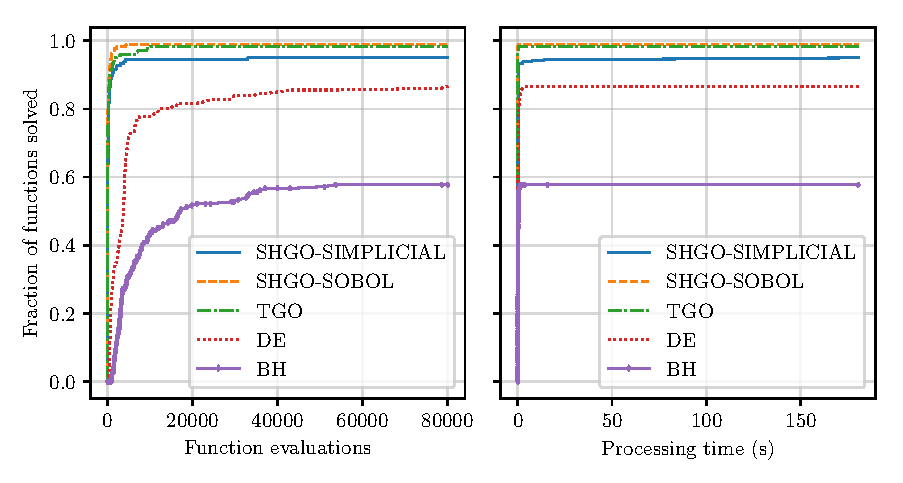
\includegraphics[scale=1.0]{./Fig12.pdf}}
{\caption{Performance profiles for SHGO, TGO, DE and BH on SciPy benchmarking test suite} \label{fig:pprofile}} 
\end{figure}

\begin{figure} %\label{fig:resmin}
\centerline{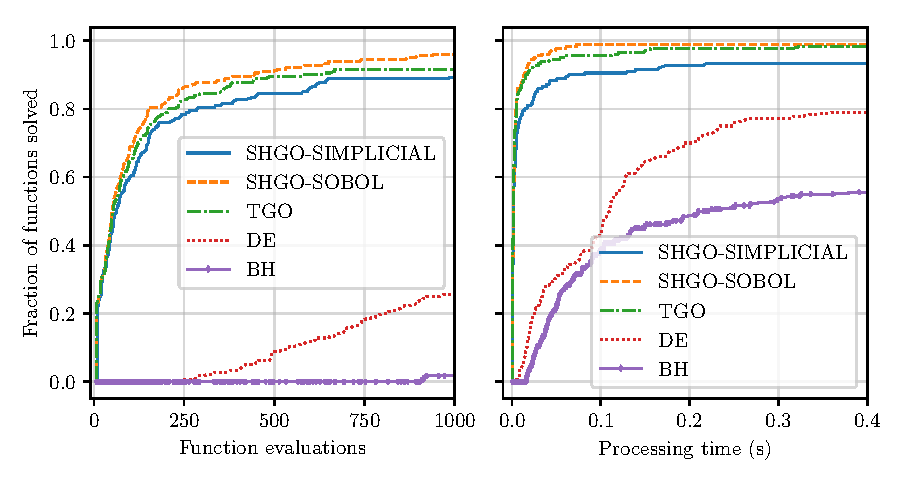
\includegraphics[scale=1.0]{./Fig13.pdf}}
{\caption{Performance profiles zoomed in to the range of $f.e.=[0, 1000]$ function evaluations and $[0, 0.4]$ seconds run time} \label{fig:pprofilezoom}} 
\end{figure}

\section{Invariance and optimum minimiser pool}
The following 4 optimisation test problems were used to demonstrate the applications of \Cref{theorem:invariance_M} and to show the minimiser pool growth compared to TGO over a large number of sampling points. The results plotted in \Cref{fig:resmin} shows that SHGO performed as expected with the minimiser pool staying at the optimum cardinality to map all the local minima once the sampling is adequate as well as the shortcomings of the TGO especially in the higher dimensional test problems where the the minimiser pool tends to grow rapidly with the number sampling points $N$.

The Ursem01 function for two dimensions is defined as follows \citep{Gavana2016}
\begin{equation} \label{eq:Ursem01}
f(\bold{x}) =  \displaystyle - \sin{\left(2 x_1  - 0.5 \pi \right) - 3 \cos{\left(x_2\right)}} - 0.5 x_1 , ~ \bold{x} \in \Omega =  [0, 9] \times [-2, 2] 
\end{equation}

The paraboloid function for six dimensions is defined as follows %\citep{Gavana2016}
\begin{equation} \label{eq:Paraboloid }
f(\bold{x}) =  \displaystyle \sum^6_{i=1} x_i^2, ~ \bold{x} \in \Omega =  [-10, 10]^6 
\end{equation}

The Bird function for two dimensions is defined as follows \citep{Gavana2016}
\begin{align} \label{eq:Bird} \nonumber
f(\bold{x}) =& \left(x_1 - x_2\right)^{2} + e^{\left[1 -
         \sin\left(x_1\right) \right]^{2}} \cos\left(x_2\right) + e^{\left[1 -
          \cos\left(x_2\right)\right]^{2}} \sin\left(x_1\right), \\ 
          &\bold{x} \in \Omega = [-2\pi, 2\pi]^2 
\end{align}


The Schwefel01 function for six dimensions is defined as follows \citep{Gavana2016}
\begin{equation} \label{eq:Schwefel01}
f(\bold{x})= \left(\sum_{i=1}^n x_i^2 \right)^{\sqrt{\pi}} , ~ \bold{x} \in \Omega = [-100, 100]^6
\end{equation}

\begin{figure} %\label{fig:resmin}
\centerline{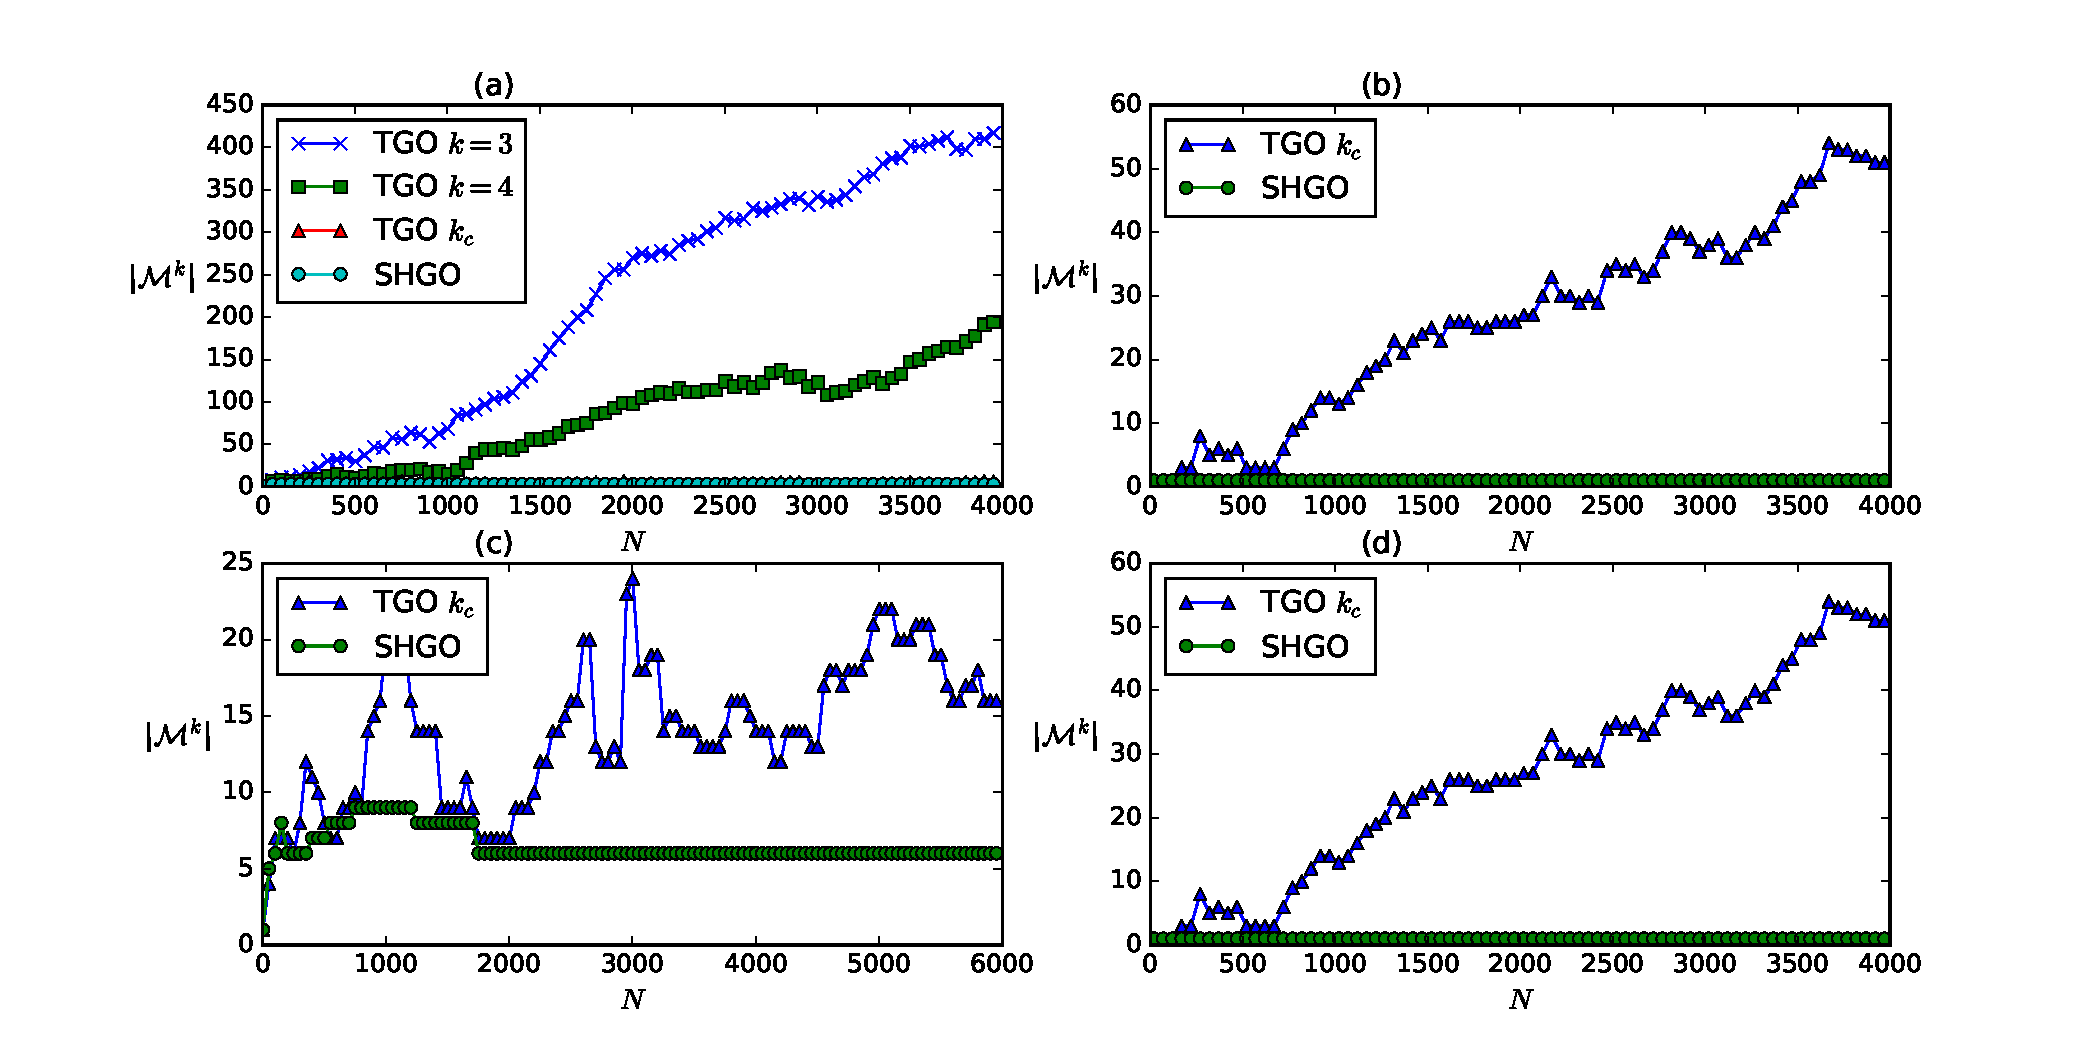
\includegraphics[scale=0.6]{./Fig11.pdf}}
{\caption{(a) The minimiser pool growth of the TGO and SHGO algorithms for the smooth objective function described in Example 3 and restated in Equation~(\ref{eq:Ursem01}) for convenience, the SHGO never increases above the optimum of $|\mathcal{M}| = 3$, for TGO 3 different values of the $k$ parameter are shown. (b) The minimiser pool growth for the six-dimensional paraboloid problem defined by Equation (\ref{eq:Paraboloid }), note that even though the problem has only one minimum, the minimiser pool for TGO set at $k = k_c$ tends to increase for increasing sampling points $N$. In general this problem is exacerbated in higher dimensions while SHGO stays at the optimum $|\mathcal{M}| = 1$. The TGO minimiser pool for $k = 3$ and $k = 4$ are not shown here because the minimiser pool grows too rapidly. (c) The minimiser pool growth for the two dimensional Bird problem defined by Equation~(\ref{eq:Bird}), an important observation here is that $|\mathcal{M}|$ is higher than optimum for SHGO before the sampling is adequate as defined by Equation~(\ref{theorem:invariance_M}) which happens at the after there are $N = 1722$ Sobol sequenced points after which $|\mathcal{M}|$ stays at the optimum value equal to the number of unique local minima with increasing $N$. (d) The minimiser pool growth for the six dimensional Schwefel01 problem defined by Equation (\ref{eq:Schwefel01}), here again $|\mathcal{M}|$ for TGO set at $k_c$ grows rapidly with $N$ while $|\mathcal{M}|$ for SHGO stays constant at the optimum.} \label{fig:resmin}} 

\end{figure}

%In the Table~\ref{tab:results} ndim = $n$ refers the the number of dimensions, nfev refers to the total number of function evaluations used to solved the problem, nlmin refers to the number of local minima found while nulmin refers to the number of local minima that are unique to a set tolerance, success refers to whether or not the algorithm successfully found the correct global minima and finally runtime is the total time the algorithm ran on an optimisation problem measured in seconds.

%\Cref{sec:nres}


%!! TODO: Lennard-Jones crystals \citep{Chill2014} where we have, using function evaluations as a metric, SHGO was 36.5 times faster than BH, 79.6 times faster than DE and 2.6 times faster than our own in-house version of TGO in solving $n = 6$, simulate for the $n=3 \times 60$ using the symmetry constraints.

%!!TODO: Move to an appendix


%\section{Conclusion}
\chapter{Concluding remarks}
The SHGO algorithm developed here shows promising properties and performance. On problems with linear constraints it was shown to provide competitive results to the TGO, Lc-DISIMPL, PSwarm and DIRECT-L1 algorithms. The use of a simplicial complex provides access to a wealth of tools from combinatorial topology and the growing field of computational homology. It is hoped that these will drive further extensions and development of the algorithm. Many challenges remain such as finding the most appropriate sampling sequences for different classes of problems, and finding computer resource-efficient triangulation schemes. Due to the useful characterisations of objective function hypersurfaces provided by the homology groups of the simplicial complex, SHGO allows an optimisation practitioner with a useful visual tool for understanding and efficiently solving higher dimensional black and grey box optimisation problems.

The main initial driving force behind the development of this algorithm grew out of a need for efficient, deterministic and reliable global optimisation methods for applications in phase equilibria modelling and calculations. However, the SHGO algorithm described here is appropriate for solving a wider class of global optimisation problems, including those where mapping all the local minima is of interest and where only the global optima is needed. It is especially appropriate for computationally expensive black and grey box functions common in science and engineering as described for example by \citet{Shan2010}.
 
Some key features of SHGO are that, when the optimisation search space is adequately sampled (or enough information is available to determine that all local minima have been mapped) then it is guaranteed that only one starting point for every locally convex domain will be produced by the algorithm. Note that in optimisation problems where the number of local minima is known, the sampling can stop and the local minimisation step started without superfluous function evaluations. However, for optimisation problems with an unknown number of local minima is unknown (and thus we can never truly know if all local minima has been found for any finite number of sampling), the guarantee still holds that that SHGO will not produce superfluous starting points that lead to the same stationary points. In addition because the homology groups can be calculated as sampling progresses an optimisation practitioner can both visualise the extent of the optimisation problem's multi-modality and use intelligent stopping criteria for the sampling stage.


%!! Offer suggestions of exploring other sampling and triangulation schemes. Also offer suggestions in useful problems and function classes to map out using shgo


% Appendix Speed up compilato
\subfile{./raw.tex}

%\include{introduction}
%\include{literature}
%\include{background}
%\include{controlanalysis}
%\include{current}
%\include{controllerdesign}
%\include{montecarlo}
%\include{program}
%\chapter{Experimental Results} \label{sec:results}
\section{Comparison to algorithms that can solve problems with linear constraints}

In this section we provide experimental comparisons on 22 linearly constrained problems comparing the SHGO, TGO, Lc-DISIMPL \citep{Paul2016}, PSwarm \citep{Vaz2008} and DIRECT-L1 \citep{finkel2003direct} algorithms. Note that the data for the Lc-DISIMPL, PSwarm and DIRECT-L1 algorithms was taken from \citet{Paul2016}. The same error of $pe = 0.01\%$ used by \citet{Paul2016} was also used in this publication. To provide a fair comparison of TGO to SHGO and the other solvers the TGO algorithm was modified to stop sampling when it produced a minimiser that lead to the global minimum of the problem. Table \ref{tab:lc_results} shows the results. Here f.e.\ is the total number of objective function evaluations required to solve the function and p.f.e. is the total number of penalty function evaluations. \citet{Paul2016} used DIRECT-L1 with the 3 different penalty parameters (p.p.) shown in the table. The PSwarm solver was run 10 times for each test problem. 

The SHGO-Simpl, SHGO-Sobol and TGO (using Henderson's formula for $k_c$) algorithms were able to solve all 22 problems. The lowest average number of function evaluations was achieved by SHGO-Simpl followed by SHGO-Sobol and TGO. It can be observed that Lc-DISIMPL-v achieved a better performance than any other algorithm for the horst-1 to horst-6, hs024, hs035, s232, s250 and bunnag2 problems. As noted in \citet{Paul2016} the initial triangulation of Lc-DISIMPL-v evaluates the function values at the vertices of the simplices and therefore for some of the tested problems the solutions were found after initial triangulation on one of the vertices of the feasible region. It is also possible to initiate SHGO with such an initial triangulation by definition the first few vertices in $\mathcal{X}$ as the intercepts of the linear constraints in a similar way to \citet{Paul2016} and then continuing to add sampling points as normal.

Table \ref{tb:lc} provides additional information for SHGO and TGO including the total number of function evaluations required by the algorithm to solve the problem (f.e.), the number of minimisers generated as starting points by the algorithm (nlmin), the number of unique local minima mapped by the algorithm (nulmin) and the total processing time (runtime) in seconds.

It can be seen that neither of the SHGO algorithms produced more starting points leading to the same local minima as predicted by the theory for adequately sampled function surfaces. On the contrary TGO produced more than one starting point in the same locally convex domain on some test problems which lead to extra function evaluations, producing a poorer overall performance. While SHGO-Simpl had the lowest number of average function evaluations, a higher processing run time is observed compared to the other 2 algorithms. This can be explained by the fact the triangulation code for the sampling has, not yet been optimised, which consumed most of the run time. SHGO-Sobol and TGO use the same sampling generation code and it is observed that SHGO-Sobol has a lower processing run time as expected.


The source code used to produce these results including the scripts that run the test benchmarking suite is publically available at \citet{SHGOpy}. The specifications of the system used to run the test problems can be found in Appendix~\ref{sec:nres}.



\setlength{\tabcolsep}{5.5pt}
\begin{landscape}
% \hspace*{-3cm} 
\begin{table}[htbp]
\caption{Function evaluation comparisons for test problems with linear constraints.}%The results for the Lc-DSIMPL, PSwarm and DIRECT-L1 algorithms were taken from \citet{Paul2016}}
%{\tablinesep=2ex\tabcolsep=10pt
\begin{tabular}{lrrrrrrrrrrrrrr}
\toprule
 & \multicolumn{1}{l}{shgo-}  & \multicolumn{1}{l}{} & \multicolumn{1}{l}{tgo}  & \multicolumn{2}{l}{Lc-DSIMPL-$^c$}   & \multicolumn{1}{l}{PSwarm$^c$} & \multicolumn{1}{l}{} & \multicolumn{1}{l}{} & \multicolumn{1}{l}{}  & \multicolumn{1}{l}{} & \multicolumn{1}{l}{} & \multicolumn{2}{l}{DIRECT-L1$^c$}  &  \\  \cmidrule(lr){7-12}
 & \multicolumn{1}{l}{-simpl}  & \multicolumn{1}{l}{-sobol} & \multicolumn{1}{l}{}  & \multicolumn{1}{l}{-v} & \multicolumn{1}{l}{-c} & \multicolumn{1}{l}{Minimum} & \multicolumn{1}{l}{} & \multicolumn{1}{l}{Average} & \multicolumn{1}{l}{} & \multicolumn{1}{l}{Maximum} & \multicolumn{1}{l}{} & \multicolumn{1}{l}{p.p. = 10} & \multicolumn{1}{l}{p.p. = 10$^2$} & \multicolumn{1}{l}{p.p.=10$^6$} \\  \cmidrule(lr){2-3} \cmidrule(lr){4-4}  \cmidrule(lr){5-6} \cmidrule(lr){7-8} \cmidrule(lr){9-10} \cmidrule(lr){11-12}  \cmidrule(lr){13-15}
Problem & \multicolumn{1}{l}{f.e.} & \multicolumn{1}{l}{f.e.} & \multicolumn{1}{l}{f.e.} & \multicolumn{1}{l}{f.e.} & \multicolumn{1}{l}{f.e.} & \multicolumn{1}{l}{f.e.} & \multicolumn{1}{l}{p.f.e} & \multicolumn{1}{l}{f.e.} & \multicolumn{1}{l}{p.f.e.} & \multicolumn{1}{l}{f.e.} & \multicolumn{1}{l}{p.f.e} & \multicolumn{1}{l}{f.e} & \multicolumn{1}{l}{f.e.} & \multicolumn{1}{l}{f.e.} \\ 
\midrule
horst-1  & 97 & 24 & 34 & \textbf{7} & 249 & 167 & 182 & 1329$^{b(3)}$ & 1343$^{b(3)}$ & 4100$^{b(3)}$ & 4101$^{b(3)}$ & 287$^a$ & 3689 & $>$100000 \\[0.05cm]
horst-2  & 10 & 11 & 11 & \textbf{5} & 171 & 160 & 176 & 424 & 492 & 768 & 867 & 265$^a$ & 10829 & $>$100000 \\[0.05cm]
horst-3  & 6 & 7 &  6 & \textbf{5} & 249 & 42 & 43 & 44 & 45 & 46 & 47 & 5$^a$ & 591 & 617 \\[0.05cm]
horst-4  & 10 & 25 & 24 & \textbf{8} & 260 & 90 & 179 & 114 & 194 & 129 & 211 & 58293$^a$ & $>$100000 & $>$100000 \\[0.05cm]
horst-5  & 20 & 15 & 15 & \textbf{8} & 259 & 106 & 150 & 134 & 192 & 214 & 302 & 7$^a$ & $>$100000 & $>$100000 \\[0.05cm]
horst-6  & 22 & 59 & 77 & \textbf{10} & 284 & 90 & 172 & 110 & 192 & 133 & 227 & 11$^a$ & 739$^a$ & $>$100000 \\[0.05cm]
horst-7  & \textbf{10} & 15 & 13 & \textbf{10} & 220 & 188 & 201 & 380 & 403 & 919 & 957 & 7$^a$ & 71$^a$ & $>$100000 \\[0.05cm]
hs021  & 24 & \textbf{23} & \textbf{23} & 189 & 133 & 110 & 110 & 189 & 192 & 392 & 405 & 97 & 97 & 97 \\[0.05cm]
hs024  & 24 & 15 & 36 & \textbf{3} & 141 & 101 & 153 & 118 & 172 & 138 & 195 & 19$^a$ & 57$^a$ & $>$100000 \\[0.05cm]
hs035  & 37 & 41 & \textbf{35} & 630 & 721 & 266 & 311 & 316 & 369 & 327 & 373 & $>$100000 & $>$100000 & $>$100000 \\[0.05cm]
hs036  & 105 & 20 & 103 & \textbf{8} & 314 & 179 & 179 & 396 & 401 & 561 & 574 & 25$^a$ & 49$^a$ & $>$100000 \\[0.05cm]
hs037  & 72 & \textbf{63} & 258 & 186 & 9129 & 127 & 131 & 160 & 167 & 201 & 574 & 7$^a$ & 7$^a$ & $>$100000 \\[0.05cm]
hs038  & \textbf{225} & 1029 & 389 & 3379 & $>$100000 & 53662 & 54445 & 58576 & 59821 & 65677 & 67660 & 7401 & 5885 & 6511 \\[0.05cm]
hs044  & 199 & 35 & 51 & \textbf{20} & 440 & 148$^{b(9)}$ & 218$^{b(9)}$ & 186$^{b(9)}$ & 281$^{b(9)}$ & 201$^{b(9)}$ & 299$^{b(9)}$ & 90283 & $>$100000 & $>$100000 \\[0.05cm]
hs076  & 56 & \textbf{37} & 44 & 548 & 4794 & 132 & 198 & 203 & 286 & 275 & 341 & 19135 & $>$100000 & $>$100000 \\[0.05cm]
s224  & 166 & 165 & 165 & \textbf{49} & 463 & 105 & 107 & 121 & 122 & 157 & 158 & 7$^a$ & 431 & 457 \\[0.05cm]
s231  & \textbf{99} & \textbf{99} & 383 & 2137 & 655 & 542 & 1011 & 2366 & 3020 & 4116 & 4800 & 1261 & 1209 & 43341 \\[0.05cm]
s232 & 24 & 15 & 22 & \textbf{3} & 141 & 105 & 144 & 119 & 171 & 162 & 236 & 19$^a$ & 57$^a$ & $>$100000 \\[0.05cm]
s250 & 105 & 20  & 103 & \textbf{8} & 314 & 296 & 296 & 367 & 375 & 495 & 498 & 25$^a$ & 49$^a$ & $>$100000 \\[0.05cm]
s251 & 72 & \textbf{63} & 258 & 186 & 9127 & 83 & 84 & 129 & 137 & 175 & 180 & 7$^a$ & 7$^a$ & $>$100000 \\[0.05cm]
bunnag1  & \textbf{34} & 47 & 39 & 630 & 721 & 132 & 142 & 214 & 228 & 411 & 438 & 1529 & 1495 & 1463 \\[0.05cm]
bunnag2  & 46 & 36 & 35 & \textbf{16} & 500 & 150 & 153 & 252 & 259 & 410 & 426 & $>$100000 & $>$100000 & $>$100000 \\[0.05cm]
\cmidrule(lr){2-15}
Average  & \textbf{66} & 88 & 100 & 366 & $>$5877 & 2590 & 2672 & 3011 & 3130 & 3637 & 3812 & $>$17213 & $>$28421 & $>$75113 \\[0.05cm]
\bottomrule
\end{tabular}
\begin{tabular}{l}
$a$ result is outside the feasible region \\
$b(t)$ $t$ out of 10 times the global solution was not reached \\
$c$ results produced by \citeauthor{Paul2016} (\citeyear{Paul2016})
\end{tabular}
%}
 \label{tab:lc_results}
\end{table}
\thispagestyle{plain}
\end{landscape}


\begin{table}[htbp]
\caption{Total and average performance over all 22 test problems.}
\begin{tabular}{llrrrr}
\toprule
    &                &  f.e. &  nlmin &  nulmin  &   runtime (s) \\
problem & name        &       &        &                  &           \\
\midrule
All & shgo-simpl     &  1463 &     26 &      26  &       0.27294 \\
    & shgo-sobol       &  1864 &     23 &      23 &       0.11225 \\
    & tgo       &  2123 &     29 &      25  &       0.093607 \\
Average & shgo-simplicial      &    65 &      1 &       1  &  0.012852 \\
    & shgo-sobol       &    88 &      1 &       1  &  0.004144 \\
    & tgo      &    100 &      1 &       1  &  0.004542 \\
\bottomrule
\end{tabular}
\label{tb:lc}
\end{table}

\section{Function evaluations and comparison to other open source global optimisation algorithms}
In this section we present numerical experiments comparing the SHGO and TGO algorithms with the SciPy implementations \citep{scipy} of basinhopping (BH) \citep{li1987monte, wales2003energy, wales1997global, wales1999global} and differential evolution (DE) \citep{Storn1997}. These algorithms were chosen both because the open source versions are readily available in the SciPy project and because BH is commonly used in energy surface optimisations \citep{Wales2015} from which the motivation for developing SHGO grew. DE has also been applied in optimising Gibbs energy surfaces for phase equilibria calculations \citep{Zhang2011}. The optimisation problems in Appendix~\ref{sec:nres} were selected from the SciPy global optimisation benchmarking test suite \citep{Adorio2005, Gavana2016, Jamil2013, Mishra2007, Mishra2006, NIST2016}. The test suite contains multi-modal problems with box constraints, they are described in detail in \citet{Gavana2016}. We again used the stopping criteria $pe = 0.01\%$ for SHGO and TGO. For the stochastic algorithms (BH and DE) the starting points provided by the test suite were used. For every test the algorithm was terminated if the global minimum was not found after 10 minutes of processing time and the test was flagged as a fail. For comparisons we used normalised performance profiles \citep{Dolan2002} using function evaluations and processing time as performance criteria. In total 180 test problems were used.

From \Cref{fig:pprofile} it can be observed that for this problem set SHGO-Sobol was the best performing algorithm, followed closely by TGO and SHGO-Simpl. \Cref{fig:pprofilezoom} provides a clearer comparison between these three algorithms. While the performance of all 3 algorithms are comparable, SHGO-Sobol tends to outperform TGO, solving more problems for a given number of function evaluations. This is expected since, for the same sampling point sequence, TGO produced more than one starting point in the same locally convex domain on some test problems which leads to extra function evaluations. In total TGO produced 403 minima of which only 393 minima were unique while all of the 225 minima produced by SHGO-Sobol were unique. SHGO-Simpl produced 238 of which all 238 were unique. It is apparent that SHGO-Simpl performed worse compared to the other sampling methods despite a better performance on the test problem set with linear constraints. There are two reasons for this result. First of all, the uniformity properties of the Sobol sequence hold only for hypercubes. Therefore, it is lost for geometries defined by the search spaces inside linear constraints. Secondly the current code for the triangulation of the simplex cannot add only one sampling point per iteration, but must split all the simplices until the symmetry of the entire complex is restored. This leads to a much higher number of function evaluations during the sampling step of the algorithm.

\Cref{tab:results} in Appendix~\ref{sec:nres} shows the raw numerical results. Note that, unlike the data in performance profiles, failed test runs did not get set to the worst case performance criteria by any solver (in order to preserve the raw data). Therefore the total and average function evaluations and processing times are misleading. The Table is mostly useful for comparisons on a particular test problem as well as comparing the total number of minima and unique minima found.



%From the results it should first be noted that not all of the 1035 starting minimisers produced by SHGO algorithm lead to unique local minima (of which  944 is found across all the problems), this is both due to the fact that the 100 initial sampling points were inadequate for many of the problems and that the local minimisation was not supplied with the set of bounds provided by the boundary of the $k-$chain around $\textrm{st}\left( v_i \right)$,  $\partial \left( C(\mathcal{H}^k) \right), k = n + 1$, and could therefore jump outside the locally convex domain in the local minimisation step. Furthermore some of the problems in the  test suite are not smooth functions. Of the 895 starting minimisers produced by TGO algorithm only 749 unique minima were found. Overall SHGO used less functions evaluations per number of unique minima discovered (123.99) compared to TGO (136.82).  However, TGO used less function evaluations overall since SHGO used more local minimisation evaluations to find more unique local minima.


\begin{figure} %\label{fig:resmin}
\centerline{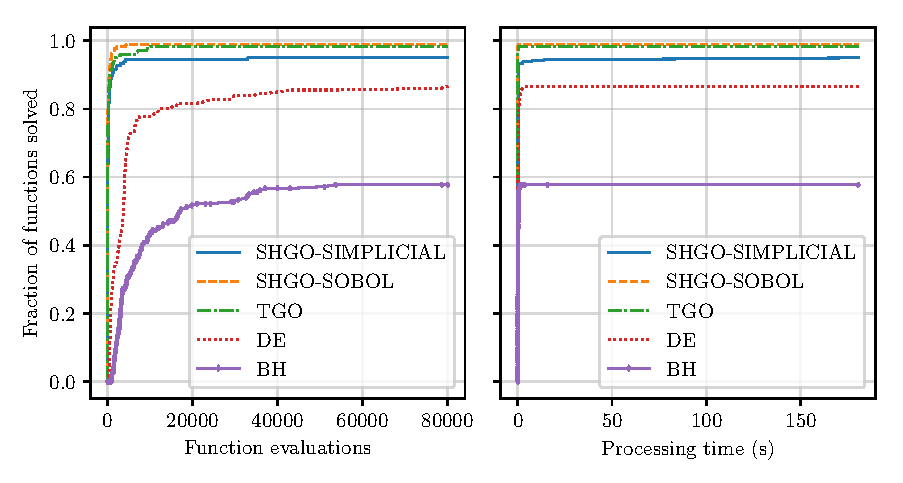
\includegraphics[scale=1.0]{./Fig12.pdf}}
{\caption{Performance profiles for SHGO, TGO, DE and BH on SciPy benchmarking test suite} \label{fig:pprofile}} 
\end{figure}

\begin{figure} %\label{fig:resmin}
\centerline{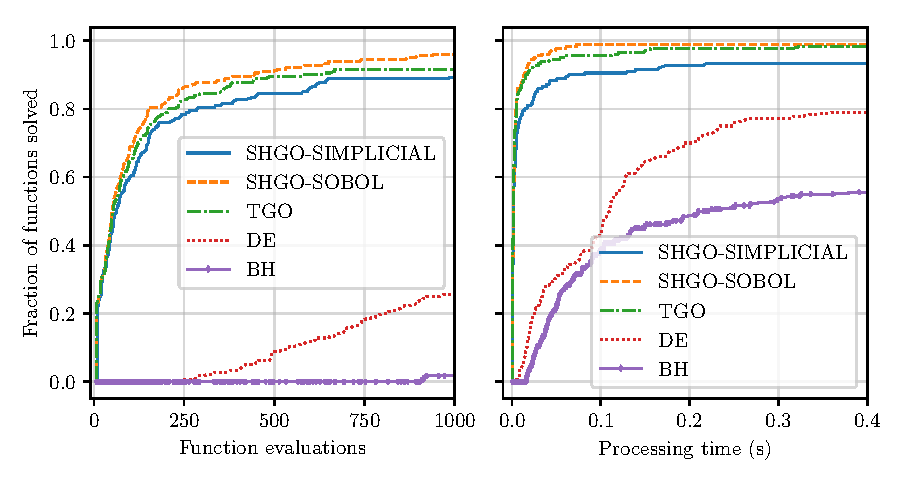
\includegraphics[scale=1.0]{./Fig13.pdf}}
{\caption{Performance profiles zoomed in to the range of $f.e.=[0, 1000]$ function evaluations and $[0, 0.4]$ seconds run time} \label{fig:pprofilezoom}} 
\end{figure}

\section{Invariance and optimum minimiser pool}
The following 4 optimisation test problems were used to demonstrate the applications of \Cref{theorem:invariance_M} and to show the minimiser pool growth compared to TGO over a large number of sampling points. The results plotted in \Cref{fig:resmin} shows that SHGO performed as expected with the minimiser pool staying at the optimum cardinality to map all the local minima once the sampling is adequate as well as the shortcomings of the TGO especially in the higher dimensional test problems where the the minimiser pool tends to grow rapidly with the number sampling points $N$.

The Ursem01 function for two dimensions is defined as follows \citep{Gavana2016}
\begin{equation} \label{eq:Ursem01}
f(\bold{x}) =  \displaystyle - \sin{\left(2 x_1  - 0.5 \pi \right) - 3 \cos{\left(x_2\right)}} - 0.5 x_1 , ~ \bold{x} \in \Omega =  [0, 9] \times [-2, 2] 
\end{equation}

The paraboloid function for six dimensions is defined as follows %\citep{Gavana2016}
\begin{equation} \label{eq:Paraboloid }
f(\bold{x}) =  \displaystyle \sum^6_{i=1} x_i^2, ~ \bold{x} \in \Omega =  [-10, 10]^6 
\end{equation}

The Bird function for two dimensions is defined as follows \citep{Gavana2016}
\begin{align} \label{eq:Bird} \nonumber
f(\bold{x}) =& \left(x_1 - x_2\right)^{2} + e^{\left[1 -
         \sin\left(x_1\right) \right]^{2}} \cos\left(x_2\right) + e^{\left[1 -
          \cos\left(x_2\right)\right]^{2}} \sin\left(x_1\right), \\ 
          &\bold{x} \in \Omega = [-2\pi, 2\pi]^2 
\end{align}


The Schwefel01 function for six dimensions is defined as follows \citep{Gavana2016}
\begin{equation} \label{eq:Schwefel01}
f(\bold{x})= \left(\sum_{i=1}^n x_i^2 \right)^{\sqrt{\pi}} , ~ \bold{x} \in \Omega = [-100, 100]^6
\end{equation}

\begin{figure} %\label{fig:resmin}
\centerline{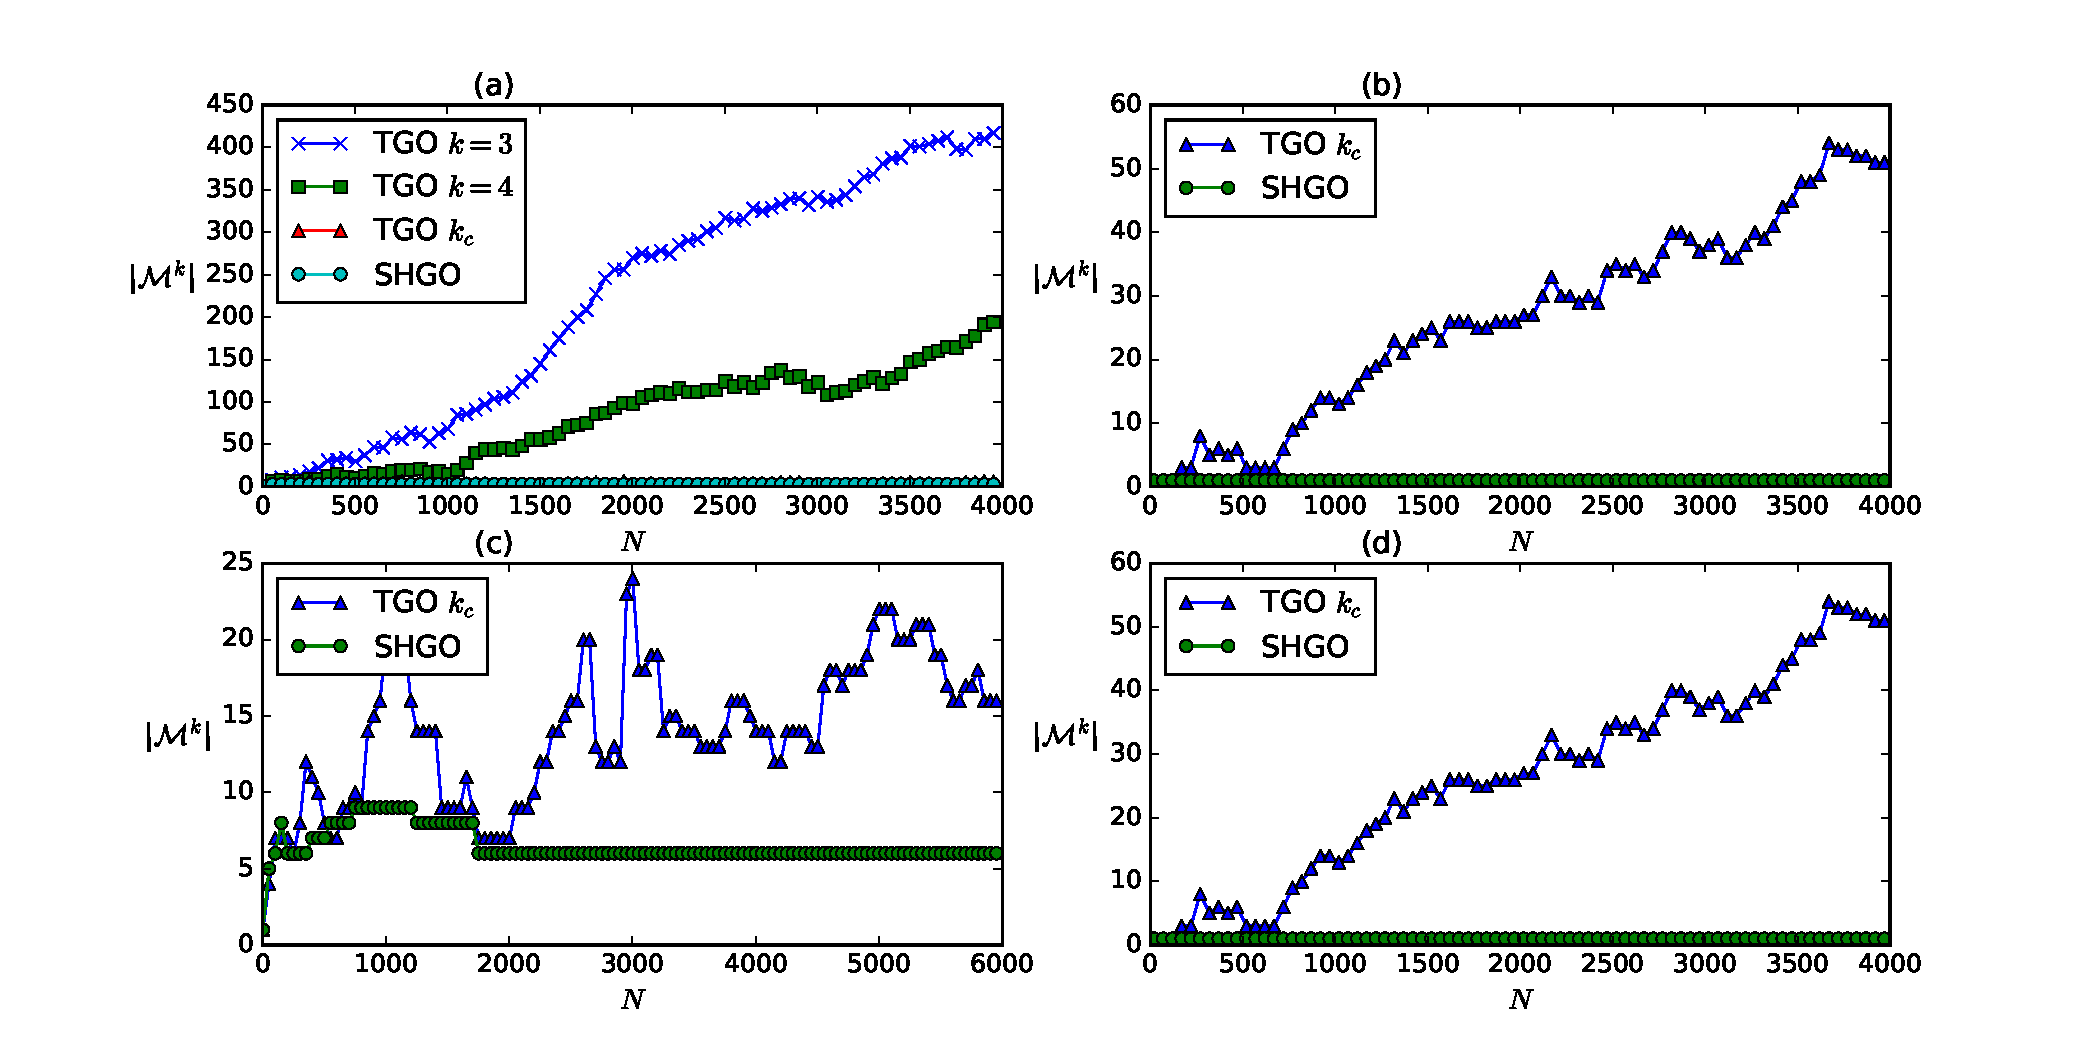
\includegraphics[scale=0.6]{./Fig11.pdf}}
{\caption{(a) The minimiser pool growth of the TGO and SHGO algorithms for the smooth objective function described in Example 3 and restated in Equation~(\ref{eq:Ursem01}) for convenience, the SHGO never increases above the optimum of $|\mathcal{M}| = 3$, for TGO 3 different values of the $k$ parameter are shown. (b) The minimiser pool growth for the six-dimensional paraboloid problem defined by Equation (\ref{eq:Paraboloid }), note that even though the problem has only one minimum, the minimiser pool for TGO set at $k = k_c$ tends to increase for increasing sampling points $N$. In general this problem is exacerbated in higher dimensions while SHGO stays at the optimum $|\mathcal{M}| = 1$. The TGO minimiser pool for $k = 3$ and $k = 4$ are not shown here because the minimiser pool grows too rapidly. (c) The minimiser pool growth for the two dimensional Bird problem defined by Equation~(\ref{eq:Bird}), an important observation here is that $|\mathcal{M}|$ is higher than optimum for SHGO before the sampling is adequate as defined by Equation~(\ref{theorem:invariance_M}) which happens at the after there are $N = 1722$ Sobol sequenced points after which $|\mathcal{M}|$ stays at the optimum value equal to the number of unique local minima with increasing $N$. (d) The minimiser pool growth for the six dimensional Schwefel01 problem defined by Equation (\ref{eq:Schwefel01}), here again $|\mathcal{M}|$ for TGO set at $k_c$ grows rapidly with $N$ while $|\mathcal{M}|$ for SHGO stays constant at the optimum.} \label{fig:resmin}} 

\end{figure}

%In the Table~\ref{tab:results} ndim = $n$ refers the the number of dimensions, nfev refers to the total number of function evaluations used to solved the problem, nlmin refers to the number of local minima found while nulmin refers to the number of local minima that are unique to a set tolerance, success refers to whether or not the algorithm successfully found the correct global minima and finally runtime is the total time the algorithm ran on an optimisation problem measured in seconds.

%\Cref{sec:nres}


%!! TODO: Lennard-Jones crystals \citep{Chill2014} where we have, using function evaluations as a metric, SHGO was 36.5 times faster than BH, 79.6 times faster than DE and 2.6 times faster than our own in-house version of TGO in solving $n = 6$, simulate for the $n=3 \times 60$ using the symmetry constraints.

%!!TODO: Move to an appendix

%\include{conclusion}

\bibliography{library}
\bibliographystyle{abbrvnat}

\appendix
%\include{programlistings}
%\include{parametervalues}
%\include{programmingdetails}
%\include{testresults}


%\bibliographystyle{cheming}
%\bibliographystyle{apalike}

%\printindex

\end{document}